%\setstretch{1.6}
\chapter{Counterexamples to Baum-Connes and Large Girth expanders.}
In this chapter we develop the basic concepts of coarse geometry for metric spaces and outline some coarse properties that can be associated to a metric space. We then outline certain analytic group and groupoid properties and connect these to their coarse counterparts. Secondly, we introduce the coarse Baum-Connes conjecture for proper metric spaces and outline machinery to construct counterexamples to this conjecture by converting the coarse assembly map into a groupoid assembly map.

We then present a unifying approach to all known counterexamples to this conjecture by developing the groupoid centric viewpoint of \cite{MR1911663} further, introducing a new conjecture known as the \textit{boundary coarse Baum-Connes conjecture}. First however we outline the construction of the algebras involved in defining the coarse assembly map $\mu$, then make some connections to groupoid equivariant KK-theory. These ideas then allow us to formulate the boundary coarse Baum-Connes conjecture and apply homological algebra techniques to connect it to the coarse Baum-Connes conjecture.

As an example of the flexibility of this new conjecture we give a proof for certain large classes of expander graph, generalising work of Willett and Yu \cite{explg1}.

\section{Coarse geometry, Groupoids and Assembly.}
In this section we outline the coarse geometry and group theoretic properties that are going to be considered throughout this document. The overall scheme of this section is first to consider some general coarse ideas associated to metric spaces and then move onto discussions of certain analytic properties held by discrete groups. We will develop these coarse ideas further by introducing abstract coarse structures and their relationship to metric spaces.

\subsection{Coarse geometry.}
The notions of coarse geometry a similar in spirit to those of topology, however the focus is on the large as opposed to the small. Recall that a function $f$ between topological spaces $X$ and $Y$ is continous if the preimage of every open set in $Y$ is open in $X$. Suppose additionally that $X$ and $Y$ are metric spaces equipped with the metric topology. Then this definition of continuous function really asks that the open neighbourhoods of a point in $Y$ have open preimage in $X$ and these are in particular going to be sets of very small diameter. 

The key idea in coarse geometry is somehow to supplant this notion of continous by replacing the occurrences of open in the definition with \textit{bounded}. We call such maps \textit{metrically proper}. If additionally suppose that the map $f$ sends sets of diameter $R$ to sets of diameter at most $S$ for some $S>0$. Then we call such a map \textit{bornologous}. Combining these two, we arrive at a definition:

\begin{definition}
Let $f:X \rightarrow Y$ be a map of metric spaces. $f$ is \textit{coarse} if it is both metrically proper and bornologous.
\end{definition}

A coarse map, intuitively, preserves the structure of a metric space on large scales. We call a pair of maps $f:X\rightarrow Y$, $g:Y\rightarrow X$ \textit{close} if there is a uniform bound $R$ such that $d(g(f(x),x)<R$ and $d(y,f(g(y))<R$. Two metric spaces $X$ and $Y$ are \textit{coarsely equivalent} if we can find maps $f:X\rightarrow Y$, $g:Y\rightarrow X$ that are both coarse such that the pair are close.  Classifying spaces by their coarse type is one of the basic goals of coarse geometry. An example where such coarse equivalences turn out to be useful is in analysing the topology of manifolds via their fundamental group; this idea also motivates the more technical coarse geometric ideas that permeate throughout Chapter 4.

\begin{lemma}(\u{S}varc - Milnor)
Let $\Gamma$ be a discrete group and let $X$ be a proper, free, cocompact $\Gamma$-space where the $\Gamma$ action is isometric. Then $X$ is coarsely equivalent to $\Gamma$.\qed
\end{lemma}

\begin{example}
Let $M$ be a closed compact manifold and let $\pi_{1}(M)=\Gamma$ be its fundamental group. Then $\Gamma$ is coarsely equivalent to $\tilde{M}$, the universal cover of $M$ by the Lemma above.
\end{example}

We introduce now another concept, similar in vein to the previous, that allows us to talk about uniformly controlled embeddings:

\begin{definition}
A map is called \textit{effectively proper} if additionally, for each $R>0$ there exists an $S>0$ such that the preimage of each ball of radius $R$ in $Y$ is contained in a ball of radius $S$ in $X$.
\end{definition}

This notion seems a little less natural than a metrically proper mapping, however it plays an important role in describing an embedding in this category. In particular, focusing on coarse embeddings, it is enough to consider pairs of maps that are effectively proper and bornlogous. The following is proved in \cite{EG-permanence}.

\begin{lemma}
Let $X$ and $Y$ be coarsely equivalent metric spaces. Then there exists $f$ and $g$ that are effectively proper and bornologous that impliment this coarse equivalence.
\end{lemma}

The notion of a coarse embedding is fundamental to the applications of this theory to topology and analysis, so we make it precise here:

\begin{definition}\label{def:FCE}
A metric space $X$ is said to admit a coarse embedding into Hilbert space $\mathcal{H}$ if there exist maps $f:X \rightarrow \mathcal{H}$,  and non-decreasing $\rho_{1},\rho_{2}:\mathbb{R}_{+} \rightarrow \mathbb{R}$ such that:
\begin{enumerate}
\item for every $x,y \in X$, $\rho_{1}(d(x,y)) \leq \Vert f(x) - f(y) \Vert \leq \rho_{2}(d(x,y))$;
\item for each $i$, we have $\lim_{r \rightarrow \infty}\rho_{i}(r) = +\infty$.
\end{enumerate}
\end{definition}

This connects to the notion of an effectively proper, bornologous map by observing that our controls (i.e the $S$'s that appear within the definitions) will pop out as the value of the control functions $\rho_{\pm}$ at $R$.

This property is exceptionally flexible; many constructions of metric spaces preserve coarse embeddability \cite{EG-permanence}. This property will be important in Chapter 4 where it plays an important role in results concerning groupoids and the coarse Baum-Connes conjecture.

\subsection{Properties of finitely generated discrete groups and \'etale groupoids.}
Via the construction of a Cayley graph, it is possible to introduce a metric to a finitely generated group that is compatable with the group structure. Many of the ideas in geometric group theory rely on computing coarse properties, such as coarse embeddings, for this metric. Additionally, coarse properties of this metric often connect to analytic properties of groups that are equivariant with respect to the group action. In the global context of understanding the Baum-Connes conjectures, for groups and groupoids, the following property plays an important role. As we primarily consider transformation groupoids, we focus the definition on them.

\begin{definition}
Let $H$ be a continous field of Hilbert spaces over $X$. we say that a transformation groupoid $G:=X\rtimes \Gamma$ acts on $H$ by affine isometries if for every $(x,g) \in G$ there exists an affine isometry $A_{(x,g)}:H_{xg}\rightarrow H_{x}$ such that:
\begin{enumerate}
\item $A_{(x,e)}$ is the identity map.
\item Whenever the elements $(x,g)$ and $(y,g^{'})$ belong to $G^{(2)}$ the maps $A_{(x,g)}$ and $A_{(y,g^{'})}$ are composable and the composition $A_{(x,g)}\circ A_{(y,g^{'})}=A_{(x,gg^{'}}$.
\item For any continous vector field $h(x)$ in $H$ and every $g \in \Gamma$ $A_{(x,g)}(h(xg))$ is a continous vector field in $H$.
\end{enumerate}
\end{definition}

This definition can be connected to cohomology and analysis via positive and negative type kernels \cite{MR2415834,MR2158394}. The role of positive and conditionally negative type kernels within group theory is well known and plays an important role in studying both anayltic and representation theoretic properties of groups \cite{MR2415834,MR1487204}. These ideas were extended to groupoids by Tu \cite{MR1703305}, and we define and consider them in that generality. Let $\G$ be a locally compact, Hausdorff groupoid.

\begin{definition}
A continuous function $F: \G \rightarrow \mathbb{R}$ is said to be of \textit{negative type} if 
\begin{enumerate}
\item $F|_{\G^{(0)}}=0$;
\item $\forall x \in \G, F(x)=F(x^{-1})$;
\item Given $x_{1},...,x_{n} \in \G$ all having the same range and $\sigma_{1},...,\sigma_{n} \in \mathbb{R}$ such that $\sum_{i}\sigma_{i}=0$ we have $\sum_{j,k}\sigma_{j}\sigma_{k}F(x_{j}^{-1}x_{k})\leq 0$.
\end{enumerate}
\end{definition}

The important feature of functions of this type is their connection to affine actions of locally compact, $\sigma$-compact groupoids, in fact:
\begin{theorem}Let $\G$ be a locally compact, Hausdorff groupoid. Then the following are equivalent \cite{MR1703305}:
\begin{enumerate}
\item There exists a proper negative type function on $\G$
\item There exists a continuous field of Hilbert spaces over $\G^{(0)}$ with a proper affine action of $\G$.
\end{enumerate}
\end{theorem}

This property has many connections to the Baum-Connes conjecture for locally compact groupoids, via the work of Tu \cite{MR1703305,MR1798599,cbcag2}, which we will discuss in detail later in the chapter. Here however we would like to remark on a connection with coarse embeddings that directly highlights why we are interested in this property.

\begin{proposition}
Let $\Gamma$ be a discrete finitely generated group. If $\Gamma$ has the Haagerup property then $\Gamma$ coarsely embeds into Hilbert space.\qed
\end{proposition}

\section{The coarse Baum-Connes conjecture.}

In this section we outline the construction of the coarse assembly map using only elementary K-theoretic methods. The exposition for this follows Chapters 5 and 8 from \cite{MR1399087}, however we could equally have developed this using the latter half of \cite{MR1817560,MR1388312}. We then connect this, via a groupoid, to a KK-theoretic formulation of the conjecture introduced by Tu \cite{MR1703305,MR1798599}.

\subsection{The algebras of locally compact and psuedolocal operators.}
Let $X$ be a locally compact Hausdorff topological space and let $\mathcal{H}$ be a Hilbert space. We say that $\mathcal{H}$ is an $X$-module if it admits a representation, by bounded linear operators, of $C_{0}(X)$. 

\begin{definition}
An $X$-module is \textit{adequate} if $\overline{C_{0}(X)\mathcal{H}}=\mathcal{H}$ and $C_{0}(X)\cap \mathcal{K(\mathcal{H}})= \lbrace 0 \rbrace$.
\end{definition}

\begin{remark}
Such an $X$-module is a suitably faithful representation of $X$ into Hilbert space: it leaves the Hilbert space invariant and acts essentially non-trivially from the perspective of index theory. By results of Voiculescu \cite{MR0415338} and Brown-Douglas-Fillmore \cite{MR0458196} it is sufficient to consider only adequate $X$-modules from the perspective of defining K-homology. In fact, it can be shown that the choice of adequate $X$-module is irrelevant for this task.
\end{remark}

Fix an adequate $X$-module $\mathcal{H}_{X}$.

\begin{definition}
Let $T \in \mathcal{B}(\mathcal{H}_{X})$. We say that $T$ is \textit{psuedolocal} if $[T,f] \in \mathcal{K}(\mathcal{H}_{X})$ for all $f \in C_{0}(X)$. If $Tf$ and $fT$ are compact for all $f \in C_{0}(X)$ we say that $T$ is \textit{locally compact}.
\end{definition}

These operators are important from the perspective of defining K-homology; the set of psuedolocal operators forms a $C^{*}$-algebra which we denote by $\mathcal{D}^{*}(X)$ and the locally compact operators form an ideal in $\mathcal{D}^{*}(X)$ that we denote by $\mathcal{C}^{*}(X)$. This gives us a short exact sequence of $C^{*}$-algebras:

\begin{equation*}
0 \rightarrow \mathcal{C}^{*}(X) \rightarrow \mathcal{D}^{*}(X) \rightarrow \frac{\mathcal{D}^{*}(X)}{\mathcal{C}^{*}(X)}\rightarrow 0
\end{equation*} 

\begin{definition}
We define the analytic K-homology $K_{*}(X)$ to be the topological K-theory group $K_{*+1}(\frac{\mathcal{D}^{*}(X)}{\mathcal{C}^{*}(X)})$.
\end{definition}

Using the properties of K-theory it is possible to prove that the functor $X \mapsto K_{*}(X)$ is covariant functor to abelian groups that satisfies the properties of a generalised homology theory that is dual to K-theory. For a detailed proof of this we refer the reader to \cite{MR1399087,MR1817560}.

\subsection{The Roe algebra and the assembly map.}

Let $X$ be a proper metric space. We fix once and for all a countable dense subset $Z$ and a separable Hilbert space $\mathcal{H}_{0}$ and we consider bounded operators $T$ on the Hilbert space $\ell^{2}(Z,\mathcal{H}_{0})$. We write $T=(T_{xy})_{x,y \in Z}$ for the "matrix" decomposition of $T$ as an operator with entries $T_{xy} \in \mathcal{B}(\mathcal{H}_{0})$. We then call $T$ \textit{locally compact} if:
\begin{enumerate}
\item $T_{xy}\in \mathcal{K}(\mathcal{H}_{0})$;
\item For every bounded subset $B \subset X$ the set:
\begin{equation*}
\lbrace (x,y)\in (B \times B) \cap (Z \times Z) | T_{xy}\not= 0 \rbrace 
\end{equation*}
is finite;
\end{enumerate} 
The propagation of an operator $T$ is defined to be:
\begin{equation*}
prop(T):= \inf \lbrace S>0 | T_{xy}=0 \mbox{ for all } x,y \in Z \mbox{ such that } d(x,y)>S \rbrace
\end{equation*}

This preamble leads us to:

\begin{definition}
The algebraic Roe algebra, denoted $\mathbb{C}[X]$, is the $*$-subalgebra of $\mathcal{B}(\mathcal{H}_{0})$ consisting of all finite propagation operators $T$ that are also locally compact. The Roe algebra, denoted $C^{*}X$, is the norm closure of the algebraic Roe algebra in the operator norm associated to the Hilbert space $\ell^{2}(Z,\mathcal{H}_{0})$.
\end{definition}

\begin{remark}
The Hilbert space $\ell^{2}(Z,\mathcal{H_{0}})$ is an adequate $X$-module \cite{explg1} and $C^{*}X = \mathcal{C}^{*}X \cap \lbrace$finite propagation operators$\rbrace$.
\end{remark}

We now consider a finite propagation version of the K-homology defined in the previous section:

\begin{definition}
Define $D^{*}(X)$ to be the intersection of the finite propagation operators on $\ell^{2}(Z,\mathcal{H_{0}})$ with $\mathcal{D}^{*}(X)$. 
\end{definition}
Similarly the finite propagation operators we defined above in $C^{*}(X)$  form an ideal in $D^{*}(X)$. So again we get a long exact sequence:
\begin{equation*}
0 \rightarrow C^{*}(X) \rightarrow D^{*}(X) \rightarrow \frac{D^{*}(X)}{C^{*}(X)}\rightarrow 0
\end{equation*} 
Remarkably, this short exact sequence connects to K-homology \cite{MR1399087,MR1817560}:
\begin{theorem}\label{Thm:Khom}
K-homology is equally well defined with finite propagation operators. That is $K_{*}(X)\cong K_{*+1}( \frac{D^{*}(X)}{C^{*}(X)})$.\qed
\end{theorem}

Essentially, this Theorem reflects that K-homology elements can be chosen to have arbitrarily small propagation.

Consider now long exact sequence in K-theory associated to the short exact sequence defined above:
\begin{equation*}
\xymatrix@=1em{
K_{0}(C^{*}(X)) \ar[r] & K_{0}(D^{*}(X)) \ar[r]& K_{0}(\frac{D^{*}(X)}{C^{*}(X)})\ar[d]^{\mu} & \\
K_{1}(\frac{D^{*}(X)}{C^{*}(X)})\ar[u]^{\mu}& K_{1}(D^{*}(X)) \ar[l]& K_{1}(C^{*}(X))\ar[l] &
}
\end{equation*}
Where the maps $\mu$ are the boundary map in K-theory. Using the identification provided by Theorem \ref{Thm:Khom} we get the following long exact sequence:
\begin{equation*}
\xymatrix@=1em{
K_{0}(C^{*}(X)) \ar[r] & K_{0}(D^{*}(X)) \ar[r]& K_{1}(X)\ar[d]^{\mu} & \\
K_{0}(X)\ar[u]^{\mu}& K_{1}(D^{*}(X)) \ar[l]& K_{1}(C^{*}(X))\ar[l] &
}
\end{equation*}
So we have constructed a map, using only the K-theory long exact sequence, that connects the K-homology of $X$ to the K-theory of the Roe algebra $C^{*}(X)$; this is the coarse assembly map.
\begin{conjecture}\label{conj:CBC1}(Coarse Baum-Connes conjecture I)
Let $X$ be a proper metric space and let $\mu: K_{*}(X) \rightarrow K_{*}(C^{*}(X))$ be boundary map defined above. Then $\mu$ is an isomorphism.
\end{conjecture}
This conjecture is slightly naive, as it is not in fact functorial under coarse maps. The left hand side, $K_{*}(X)$ is a topological homology theory, functorial under proper continous maps (see Chapter 5 of \cite{MR1399087}), whilst the right hand side is a coarse invariant. However, there are still positive results \cite{MR1388312}:

\begin{theorem}
Let $X$ be a uniformly contractible simplicial complex of bounded geometry. Then the coarse Baum-Connes conjecture I is true for $X$.
\end{theorem}

In order to improve the conjecture we rely on making the left hand side term $K_{*}(X)$ functorial under coarse maps. To do this we \textit{coarsen} $X$.

\begin{definition}
A \textit{coarsening} of $X$ is uniformly contractible space $\underline{E}X$ that is equipped with a coarse equivalence $X \rightarrow \underline{E}X$. 
\end{definition}

A coarsening should be thought of a classifying space associated to $X$. Below we construct the coarsening we will rely on for the rest of the document.

\begin{example}
(Rips complex) Fix $R>0$. Then the \textit{Rips complex on scale $R$} is a simplicial complex $P_{R}(X)$, where a set of points $\lbrace x_{1},...,x_{n} \rbrace$ spans a simplex if and only if $d(x_{i},x_{j}) \leq R$ for every $i,j$. If $S>R$, then every $R$ simplex will certainly be an $S$ simplex - so we have inclusions $P_{R}(X)\hookrightarrow P_{S}(X)$. Additionally these inclusions are proper. As the inclusion of $X \hookrightarrow P_{R}(X)$ induces a coarse equivalence for each $R>0$, the direct limit: $\bigcup_{R>0}P_{R}(X)$, the simplex on $X$, is a coarsening of $X$.
\end{example}

\begin{definition}
Define the coarse K-homology of $X$, denoted by $KX_{*}(X)$ to be the K-homology of any coarsening $K_{*}(\underline{E}X)$.
\end{definition}

Let $X$ be a proper metric space and by considering Rips complexes, we can compute the coarse K-homology as a direct limit:
\begin{equation*}
KX_{*}(X) = \lim_{R>0}K_{*}(P_{R}(X))
\end{equation*}
Additionally, as the K-theory of $C^{*}(X)$ is functorial under coarse maps, we get a natural coarsened version of Conjecture \ref{conj:CBC1} by considering the direct limit of the maps $\mu_{R}: K_{*}(P_{R}(X)) \rightarrow K_{*}(C^{*}(P_{R}(X))=K_{*}(C^{*}(X))$.
\begin{conjecture}\label{conj:CBC2}(The coarse Baum-Connes conjecture II).
Let $X$ be a proper metric space. Then the coarse assembly map: $\mu_{\infty}:KX_{*}(X)= \lim_{R}K_{*}(P_{R}(X)) \rightarrow K_{*}(C^{*}(X))$ is an isomorphism. 
\end{conjecture}

As before there are broadly positive results to this conjecture. The following is a striking result of Guoliang Yu concerning coarsely embeddable spaces \cite{MR1728880}:
\begin{theorem}
Let $X$ be a proper metric space that admits a coarse embedding into Hilbert space. Then the coarse Baum-Connes conjecture II is true for $X$ 
\end{theorem}
Later in the Chapter we will explore counterexamples to this conjecture by rephrasing it using groupoids. Lastly, consider a discrete group $\Gamma$ acting on a space $X$ properly, freely and cocompactly. Then we can consider the following algebras:

\begin{definition}
Let $T$ be an operator on $\ell^{2}(X,\mathcal{H}_{0})$. Then $T$ is $\Gamma$-invariant if for all $g \in \Gamma$ the matrix entries $T_{x,y}$ and $T_{gx,gy}$ are equal. Denote by $\mathbb{C}[X]^{\Gamma}$ the collections of operators that are finite propagation, locally compact and $\Gamma$-invariant. Similarly, denote $\mathbb{D}(X)^{\Gamma}$ the operators that are finite propagation, psuedolocal and $\Gamma$-invariant. Lastly, denote their completions by $C^{*}X^{\Gamma}$ and $D^{*}(X)^{\Gamma}$.
\end{definition}

These algebras also fit into the same short exact sequence, as $C^{*}X^{\Gamma}$ is an ideal in $D^{*}(X)^{\Gamma}$, just as above. This allows us to compute the K-theory long exact sequence:
\begin{equation*}
\xymatrix@=1em{
K_{0}(C^{*}(X)^{\Gamma}) \ar[r] & K_{0}(D^{*}(X)^{\Gamma}) \ar[r]& K_{1}^{\Gamma}(X)\ar[d]^{\mu} & \\
K_{0}^{\Gamma}(X)\ar[u]^{\mu}& K_{1}(D^{*}(X)^{\Gamma}) \ar[l]& K_{1}(C^{*}(X)^{\Gamma})\ar[l] &
}
\end{equation*}
We define the equivariant K-homology of $X$, denoted by $K_{*}^{\Gamma}(X)$ to be the K-theory of $K_{*+1}(\frac{D^{*}(X)^{\Gamma}}{C^{*}(X)^{\Gamma}}).$  Now the boundary maps become the equivariant coarse assembly map for the action of $\Gamma$ on $X$. By virtue of the following lemma (for a proof see \cite{explg1}), we can simplify this further.

\begin{lemma}
If the action of $\Gamma$ on $X$ is cocompact in addition to being free and proper then there is a Morita Equivalence between $C^{*}X^{\Gamma}$ and $\mathcal{K}(\ell^{2}(X))\otimes C^{*}_{r}(\Gamma)$.
\end{lemma}

This gives us, using the boundary maps, assembly maps $K_{*}^{\Gamma}(P_{R}(X)) \rightarrow K_{*}(C^{*}(P_{R}(X))^{\Gamma}) \cong K_{*}(C^{*}(X)^{\Gamma})$.

After coarsening and taking a direct limit this gives us the Baum-Connes conjecture for the discrete group $\Gamma$:

\begin{conjecture}(Baum-Connes conjecture)
Let $\Gamma$ be a finitely generated discrete group and let $\underline{E}\Gamma$ be its classifying space for proper actions. Then the map by taking direct limits of the maps defined above: $\mu: K_{*}^{\Gamma}(\underline{E}\Gamma) \rightarrow K_{*}(C^{*}_{r}(\Gamma))$ is an isomorphism.
\end{conjecture}

There are also positive results in this setting \cite{MR1487204}:

\begin{theorem}
Let $\Gamma$ be a discrete group. If $\Gamma$ has the Haagerup property then the Baum-Connes conjecture defined above holds for $\Gamma$.
\end{theorem}

This provides the connection between analysis on groups and coarse geometry.

\section{The Coarse Groupoid of a Metric Space}\label{Sect:CG}

Let $X$ be a uniformly discrete bounded geometry (sometimes denoted uniformly locally finite) metric space. We want to define a groupoid with property that it captures the coarse information associated to $X$: that will allow us to prove results about the coarse Baum-Connes conjecture.

To do this effectively we need to define the what we mean by a ``coarse structure" associated to a metric. The details of this can be found in \cite{MR2007488}.

\begin{definition}
Let $X$ be a set and let $\mathcal{E}$ be a collection of subsets of $X \times X$. If $\mathcal{E}$ has the following properties:
\begin{enumerate}
\item $\mathcal{E}$ is closed under finite unions;
\item $\mathcal{E}$ is closed under taking subsets;
\item $\mathcal{E}$ is closed under the induced product and inverse that comes from the groupoid product on $X \times X$.
\item $\mathcal{E}$ contains the diagonal
\end{enumerate}
Then we say $\mathcal{E}$ is a \textit{coarse structure} on $X$ and we call the elements of $\mathcal{E}$ \textit{entourages}. If in addition $\mathcal{E}$ contains all finite subsets then we say that $\mathcal{E}$ is \textit{weakly connected}.
\end{definition}

For a given family of subsets $\mathcal{S}$ of $X \times X$ be can consider the smallest coarse structure that contains $\mathcal{S}$. This is the coarse structure generated by $\mathcal{S}$. We can use this to give some examples of coarse structures.

\begin{example}\label{ex:MCS}
Let $X$ be a metric space. Then consider the collection $\mathcal{S}$ given by the $R$-neighbourhoods of the diagonal in $X\times X$; that is, for every $R>0$ the set:
\begin{equation*}
\Delta_{R}=\lbrace (x,y) \in X \times X | d(x,y)\leq R \rbrace
\end{equation*}
Then let $\mathcal{E}$ be the coarse structure generated by $\mathcal{S}$. This is called the \textit{metric coarse structure} on $X$. It is a uniformly locally finite proper coarse structure that is weakly connected when $X$ is a uniformly discrete bounded geometry (proper) metric space.
\end{example}

\begin{definition}
Let $X$ be a coarse space with a coarse structure $\mathcal{E}$ and consider $\mathcal{S}$ a family of subsets of $\mathcal{E}$. We say that $\mathcal{E}$ is generated by $\mathcal{S}$ if every entourage $E \in \mathcal{E}$ is contained in a finite union of subsets of $\mathcal{S}$.
\end{definition}

\begin{example}\label{ex:GACS}
Let $G$ be a group and let $X$ be a right $G$-set. Define:
\begin{equation*}
\Delta_{g}=\lbrace (x,x.g) | x \in X \rbrace  
\end{equation*}
We call the coarse structure generated by the family $\mathcal{S}:=\lbrace \Delta_{g} | g\in G\rbrace$ the \textit{group action coarse structure} on $X$. If $X$ is not a connected space; consider for example a space of graphs $X=\sqcup X_{i}$, the group action coarse structure need not be weakly connected.
\end{example}

In the situation that $X$ admits a transitive $G$-action by translations, the group action coarse structure generates the metric coarse structure. 

To build a groupoid from the metric coarse structure on $X$ we consider extensions of the pair product on $X \times X$. The most natural way to do this is by making use of the entourages arising from the metric. The approach to this problem is through Corollary 10.18 of \cite{MR2007488}, which we record as the following Lemma:

\begin{lemma}\label{Lem:CorRoe}
Let $X$ be a uniformly discrete bounded geometry metric space and let $E$ be any entourage. Then the inclusion $E \rightarrow X \times X$ extends to an injective continuous map $\overline{E} \rightarrow \beta X \times \beta X$, where $\overline{E}$ denotes the closure of $E$ in $\beta(X \times X)$.
\end{lemma}
Now we can make the definition of the coarse groupoid $G(X)$:
\begin{theorem}(\cite[Theorem 10.20]{MR2007488})
Let $X$ be a coarse space with uniformly locally finite, weakly connected coarse structure $\mathcal{E}$. Define $G(X):=\cup_{E\in \mathcal{E}}\overline{E}.$ Then $G(X)$ is a locally compact, \'etale groupoid with the induced product, inverse and topology from $\beta X \times \beta X$.
\end{theorem}
As we are considering the metric coarse structure we can reduce this to considering only generators:
\begin{equation*}
G(X):=\bigcup_{R>0}\overline{\Delta_{R}}
\end{equation*}
The following is an integral part of \cite{MR1905840} and proofs of the quoted results can be found in \cite{MR2007488}.
\begin{theorem}
Let $X$ be a uniformly discrete bounded geometry metric space. Then following hold:
\begin{enumerate}
\item $G(X)$ is an \'etale locally compact Hausdorff principal topological groupoid with unit space $G(X)^{(0)}=\beta X$. \cite[Theorem 10.20]{MR2007488}\cite[Proposition 3.2]{MR1905840};
\item $C^{*}_{r}(G(X))$ is isomorphic to the uniform Roe algebra $C^{*}_{u}(X)$. \cite[Proposition 10.29]{MR2007488};
\item The coarse Baum-Connes conjecture for $X$ is equivalent to the Baum-Connes conjecture for $G(X)$ with coefficients in $\ell^{\infty}(X,\mathcal{K})$. \cite[Lemma 4.7]{MR1905840}.
\end{enumerate}
\end{theorem}

So this lets us appeal to the theory of groupoids to conclude coarse information about a given metric space $X$. In fact, this is precisely the strategy of \cite{MR1911663} when it comes to dealing with counterexamples to the coarse Baum-Connes conjecture.

\section{Equivariant KK-theory for groupoids and assembly.}
We recall the definitions of groupoid equivariant KK-theory. For this section let $G$ be a locally compact, $\sigma$-compact, Hausdorff groupoid with Haar system. The basic notion here is that of a $G$-$C^{*}$-algebra:
\begin{definition}
A $C^{*}$-algebra $A$ is called a $G$-$C^{*}$-algebra if it is a $C_{0}(G^{(0)})$-algebra and admits a $G$-action, that is:
\begin{enumerate}
\item there is a $*$-homomorphism $\theta: C_{0}(G^{(0)}) \rightarrow Z(M(A))$ such that $\theta(C_{0}(G^{(0)}))A = A$
\item there is an isomorphism from $\alpha: s^{*}A \rightarrow r^{*}A$ such that for each $(g,h) \in G^{(2)}$ the morphisms $\alpha(g):A_{s(g)} \rightarrow A_{r(g)}$ satisfy $\alpha(g)\circ \alpha(h) = \alpha(gh)$
\end{enumerate}
We are going to be concerned with \textit{proper} $G$-algebras. Let $Z$ be a $G$-space, then under the previous definition a $Z\rtimes G$-algebra is both a $G$-algebra and a $C_{0}(Z)$-algebra, with compatability between the two structures. We then say a $G$-algebra $A$ is proper if there exists a proper $G$-space $Z$ such that $A$ is a $Z\times G$-algebra.
\end{definition}

In this context we can also extend the action of the groupoid $G$ from a $G$-algebra $A$ to any Hilbert module $E$ over $A$. See \cite{MR1798599} for more details.

\begin{definition}($KK_{G}$-cycles) \cite{MR1686846,MR1703305,MR1798599}.
Let $A$ and $B$ be $G$-algebras. Then a Kasparov $(A,B)$ $G$ equivariant bimodule consists of a triple $(E,\phi, F)$ where $E$ is a $G$-$C^{*}$-equivariant, $\mathbb{Z}/2\mathbb{Z}$-graded $B$-module, $\phi: A \rightarrow \mathcal{L}(E)$ is a $G$-equivariant $*$-homomorphism and $F\in \mathcal{L}(E)$ is of degree 1 and satisfies, for all $a \in A$ and $a_{1} \in r^{*}A$:
\begin{enumerate}
\item $a(F - F^{*}) \in \mathcal{K}(E)$
\item $a(F^{2}- 1) \in \mathcal{K}(E)$
\item $[a,F] \in \mathcal{K}(E)$
\item $a_{1}(V(s^{*}F)V^{*}-r^{*}F) \in r^{*}\mathcal{K}(E)$, where $V$ denotes the unitary operator that impliments the action of $G$ on $E$.
\end{enumerate}
Then we denote by $KK_{G}(A,B)$ the group of homotopy classes of Kasparov $(A,B)$ $G$-equivariant bimodules. 
\end{definition}

This theory has many of the same features as the more traditional non-equivariant $KK$ groups, namely:
\begin{itemize}
\item $KK_{G}(A,B)$ is covariant in second variable and contravariant in the second;
\item Bott peroidicity holds for this theory; define: $KK_{G}^{n}(A,B)=KK_{G}(A,B\otimes C_{0}(\mathbb{R}^{n}))$, then $KK_{G}^{n}(A,B)=KK_{G}^{n+2}(A,B)$;
\item For any $G$-algebra $D$ there is a natural transformation:
\begin{equation*}
\sigma_{G^{(0)},D}: KK_{G}(A,B) \rightarrow KK_{G}(A\otimes_{C_{0}(G^{(0)})}D,B\otimes_{C_{0}(G^{(0)})}D).
\end{equation*}
\item There is a natural associative product, which is compatable with $\sigma_{G^{(0)},-}$ in the obvious way.
\item There are descent morphisms compatible with the product:
\begin{eqnarray*}
\item j_{G,(red)}:KK_{G}(A,B) \rightarrow KK_{G}(A\rtimes_{(red)}G,B\rtimes_{(red)}G)
\end{eqnarray*}
\end{itemize} 

The interest in understanding proper $G$-spaces is motivated by the construction of topological $K$-theory, a homology theory on groupoids, in this context.

\begin{definition}
A \textit{classifying space for proper actions} of $G$ is a proper $G$-space $\underline{E}G$ such that for any proper $G$-space $Z$ there exists a $G$-equivariant map $Z \rightarrow \underline{E}G$ that is unique up to $G$-homotopy.
\end{definition}

Such a space always exists \cite[Section 11]{MR1703305} and one example of a model for this is given by a collection of positive measures on $G$ \cite{MR1703305}. This construction can also be given the structure of a $G$-simiplical complex \cite{cbcag2}. 

\begin{definition}($K^{top}$)
Let $G$ be a locally compact, $\sigma$-compact Hausdorff groupoid with Haar system and let $\underline{E}G$ be its classifying space for proper actions. Then we define:
\begin{equation*}
K^{top}(G,B)=\lim_{Y \subseteq \underline{E}G}KK_{G}(C_{0}(Y),B)
\end{equation*}
where the limit runs through all possible $G$-compact subspaces $Y$. If one takes $B=C_{0}(G^{(0)})$ then we denote by $K^{top}(G)$ \textit{the topological K-theory of $G$}.
\end{definition}

\begin{remark}
For a $G$-compact, proper $G$-space $Y$ we can define an assembly map by composing the descent morphism by a suitable partition associated to a proper $G$-space, that is:
\begin{equation*}
KK_{G}(C_{0}(Y),B) \rightarrow_{j_{G,red}} KK(C_{0}(Y)\rtimes_{r}G, B\rtimes_{r} G) \rightarrow K_{*}(B\rtimes_{r}G)
\end{equation*}
By taking limits through $G$-compact subspaces, one arrives at a map:
\begin{equation*}
\mu_{*}:K^{top}_{*}(G,B)\rightarrow K_{*}(B\rtimes_{r}G).
\end{equation*}
This is the Baum-Connes assembly map for $G$ with coefficients in $B$. The Baum-Connes conjecture asks if this map is an isomorphism for all possible $G$-algebras $B$, and is known in this context to have counterexamples \cite{MR1911663}, some of which arise from coarse geometry.
\end{remark}

We now return to the coarse groupoid $G(X)$ of a uniformly discrete bounded geometry metric space $X$. We recall that this groupoid is \'etale, locally compact, $\sigma$-compact. Hence we can define $KK_{G(X)}(A,B)$ for any pair of $G(X)$-algebras $A,B$. 

\begin{definition}
Let $X$ be a coarse space with a uniformly locally finite coarse structure $\mathcal{E}$ and $G(\mathcal{E})$ the coarse groupoid. For each $E \in \mathcal{E}$ we define $P_{E}(X)$ to be the simplical complex in which each finite subset $F \subset E$ spans a simplex. We denote by $P_{E}(G(\mathcal{E})$ the closure of $P_{E}(X)\times X$ in the weak $*$-topology in the dual of $C_{c}(G(\mathcal{E})$ (viewing each element of $P_{E}(X)$ as a positive measure in the obvious way).
\end{definition}

\begin{definition}
Let $X$ be a coarse space. The coarse K-homology of $X$, denoted $KX_{*}(X)$ is defined to be the directed limit: $\lim_{E \in \mathcal{E}}KK(C_{0}(P_{E}(X)),\mathcal{C})$
\end{definition}

\begin{remark}
\begin{itemize}
\item If $X$ is a uniformly discrete bounded geometry metric space and $\mathcal{E}$ is the metric coarse structure, then the $P_{\Delta_{R}}(X)$ are equal to the standard Rips complex $P_{R}(X)$.
\item The limit through the directed set of entourages $E \in \mathcal{E}$ of the $P_{E}(X)$ is a coarsening of $X$ \cite{MR1399087}. Similarly the limit of the $P_{E}(G(X))$ is a model of $\underline{E}G(X)$.
\item Lemma 4.7 in \cite{MR1905840} proves that the inclusion of a point $\lbrace x \rbrace$ viewed as a subgroupoid of $G(X)$ gives rise to a restriction map in KK-theory and this map induces an isomorphism:
\begin{equation*}
KK_{G(X)}(C_{0}(P_{E}(G(X)),\ell^{\infty}(X,\mathcal{K})) \cong KK(C_{0}(P_{E}(X)),\mathbb{C}).
\end{equation*}
Taking limits, gives us:
\begin{equation*}
K^{top}(G(X),\ell^{\infty}(X,\mathcal{K})) \cong KX_{*}(X).
\end{equation*}
\item The content of Lemma 4.4 from \cite{MR1905840} is that $\ell^{\infty}(X,\mathcal{K}) \rtimes_{r} G(X) \cong C^{*}X$. Hence, we can use the assembly map defined above for $G(X)$ with coefficients in $\ell^{\infty}(X,\mathcal{K})$ to define:
\begin{equation*}
\mu_{*}:K^{top}_{*}(G(X),\ell^{\infty}(X,\mathcal{K})) \rightarrow K_{*}(\ell^{\infty}(X,\mathcal{K})\rtimes_{r}G(X)).
\end{equation*}
This map is equivalent to the traditional coarse assembly map:
\begin{equation*}
\mu_{*}KX_{*}(X)\rightarrow K_{*}(C^{*}X).
\end{equation*}
\end{itemize}
\end{remark}

One flexibility that the groupoid picture provides is the ability to consider natural maps associated to saturated subsets. We outline a technical Lemma of Tu concerning equivariant KK-theory associated to saturated subsets required to build a long exact sequence in the topological K-theory associated to a groupoid decomposition.

\begin{lemma}
Let $G$ be a locally compact, second countable, proper groupoid with a Haar system and let $Z$ be a second countable $G$-space. If $F$ is a closed saturated subset and $U$ is its open complement then for any $G-C^{*}$-algebra $A$ there is a long exact sequence:
\begin{equation*}
\xymatrix@=1em{
KK_{G}(C_{0}(U),A) \ar[r] & KK_{G}(C_{0}(Z),A) \ar[r]& KK_{G}(C_{0}(F),A)\ar[d] & \\
KK^{1}_{G}(C_{0}(F),A)\ar[u]& KK^{1}_{G}(C_{0}(Z),A)) \ar[l]& KK^{1}_{G}(C_{0}(U),A)\ar[l] &
}
\end{equation*}
\end{lemma}

Choosing $Z$ to be a model of $\underline{E}G$, gives us a long exact sequence in K-homology associated to any closed saturated subset $F$ and coefficient algbera $A$ that naturally connects to the assembly maps $\mu, \mu_{F}, \mu_{U}$.

\section{Counterexamples to the coarse Baum-Connes conjecture and Boundary Groupoids}\label{Sect:CE}

Throughout this section let $G$ be an \'etale, Hausdorff locally compact topological groupoid. These are essentially unnecessary assumptions but we will only require groupoids in this class to fit with the coarse picture we are interested in. We follow \cite{MR1911663}. Let $F$ be a closed saturated subset of $G^{(0)}$.

We remark also that the compliment $F^{c}$ is an open saturated set. This gives rise to the algebraic decomposition:
\begin{equation*}
G = G_{F^{c}}\sqcup G_{F}
\end{equation*}
This lets us construct maps on the $*-$algebras of compactly supported functions associated with $G$,$G_{F}$ and $G_{F^{c}}$:
\begin{equation*}
0 \rightarrow C_{c}(G_{F^{c}}) \rightarrow C_{c}(G) \rightarrow C_{c}(G_{F}) \rightarrow 0.
\end{equation*}
By the properties of the maximal $C^{*}$-norm this extends to the maximal groupoid $C^{*}$-algebras:
\begin{equation*}
0 \rightarrow C_{max}^{*}(G_{F^{c}}) \rightarrow C_{max}^{*}(G) \rightarrow C_{max}^{*}(G_{F}) \rightarrow 0.
\end{equation*}
On the other hand this may fail to be an exact sequence when we complete in the norm that arises from any specific representation, for example the left regular representation $\lambda_{G}$; this can be detected at the level of K-theory, as discussed in \cite{MR1911663}, by considering the sequence:
\begin{equation}\label{eqn:neim}
K_{0}(C^{*}_{r}(G_{U}))\rightarrow K_{0}(C^{*}_{r}(G)) \rightarrow K_{0}(C^{*}_{r}(G_{F}))
\end{equation}

This was used in \cite{MR1911663} to construct multiple different types of counterexample to the Baum-Connes conjecture for groupoids - each of which invokes the following Lemma:
\begin{lemma}\label{Lem:Lemma1}(\cite[Lemma 1]{MR1911663})
Assume the sequence (\ref{eqn:neim}) is not exact at its middle term.
\begin{enumerate}
\item If the Baum-Connes map $K_{0}^{top}(G_{F}) \rightarrow K_{0}(C^{*}_{r}(G_{F}))$ is injective then the Baum-Connes map $K_{0}^{top}(G) \rightarrow K_{0}(C^{*}_{r}(G))$ fails to be surjective.
\item If the map $K_{0}(C^{*}_{max}(G_{F})) \rightarrow K_{0}(C^{*}_{r}(G_{F}))$ is injective then the map $K_{0}(C^{*}_{max}(G)) \rightarrow K_{0}(C^{*}_{r}(G))$ fails to be surjective and a fortiori the Baum-Connes map $K_{0}^{top}(G) \rightarrow K_{0}(C^{*}_{r}(G))$ fails to be surjective.
\end{enumerate}
\end{lemma}

We observe that we make is that whilst the sequence:
\begin{equation*}
\xymatrix{
0 \ar[r] & C_{r}^{*}(G_{F^{c}}) \ar[r]^{\alpha}& C_{r}^{*}(G) \ar[r]^{q} & C_{r}^{*}(G_{F}) \ar[r] & 0
}
\end{equation*}
may fail to be exact in the middle term the maps $\alpha$ and $\q$ both exist and we can see that the map $q$ is also surjective by considering the following diagram.
\begin{equation*}
\xymatrix{C^{*}_{max}(G) \ar@{->>}[r] \ar@{->>}[d] & C^{*}_{max}(G_{F}) \ar@{->>}[d]\\
C^{*}_{r}(G)\ar@{->}[r] &   C^{*}_{r}(G_{F})
}
\end{equation*}
It is also clear that the image of $\alpha$ is contained in the kernel of $q$, whence we can make the sequence exact artificially by replacing $C_{r}^{*}(G_{F^{c}})$ by the ideal $I:=\ker(q)$. We can then define a new assembly map in the first term to be the composition of the original assembly map $\mu_{F^{c}}$ and the K-theory map induced by inclusion $i_{*}:K_{*}(C^{*}_{r}(G_{F^{c}})) \rightarrow K_{*}(I)$. Then in terms of assembly maps this gives us a new commutative diagram:
\begin{equation*}\label{Fig:F1}
\xymatrix@=1em{
\ar[r] & K_{1}(C^{*}_{r}(G_{F}) \ar[r] & K_{0}(I) \ar[r]& K_{0}(C^{*}_{r}(G)) \ar[r]& K_{0}(C^{*}_{r}(G_{F})\ar[r] & K_{1}(I) \ar[r] & \\
\ar[r] & K_{1}^{top}(G_{F}) \ar[r] \ar[u]& K_{0}^{top}(G_{F^{c}}) \ar[r]\ar[u]& K_{0}^{top}(G) \ar[r]\ar[u]& K_{0}^{top}(G_{F}) \ar[r]\ar[u]& K_{1}^{top}(G_{F^{c}})\ar[u] \ar[r]& 
}
\end{equation*}
where the rows here are exact. 

As in \cite{MR1911663} we would now choose suitable groupoids $G$ and subsets $F$ of the unit space $G^{(0)}$ that allow us to use the above sequence to analyse the Baum-Connes conjecture for the groupoid $G$. We have in mind the suitation that $G=G(X)$, the coarse groupoid associated to some uniformly discrete bounded geometry metric space $X$.

\subsection{The Coarse Groupoid Conjecture}
Let $X$ be a uniformly discrete bounded geometry metric space. From what was described above we can associate to each closed saturated subset $F$ of the unit space space $\beta X$ a long exact sequence in K-theory. We consider the obvious closed saturated subset: $\partial \beta X \subset G(X)^{(0)}$. This gives us the following commutative diagram (omitting coefficients):
\begin{equation*}
\xymatrix@=1em{
\ar[r] & K_{1}(C^{*}_{r}(G(X)|_{\partial\beta X}) \ar[r] & K_{0}(I) \ar[r]& K_{0}(C^{*}_{r}(G(X))) \ar[r]& K_{0}(C^{*}_{r}(G(X)|_{\partial\beta X})\ar[r] & K_{1}(I)\ar[r] &  \\
\ar[r] & K_{1}^{top}(G(X)|_{\partial\beta X}) \ar[r] \ar[u]& K_{0}^{top}(X \times X) \ar[r]\ar[u]& K_{0}^{top}(G(X)) \ar[r]\ar[u]& K_{0}^{top}(G(X)|_{\partial\beta X}) \ar[r]\ar[u]^{\mu_{bdry}}& K_{1}^{top}(X \times X)\ar[u]\ar[r] &
}
\end{equation*}

We can now properly formulate the boundary conjecture (replacing the coefficients):

\begin{conj}\label{MC:S1} [Boundary Coarse Baum-Connes Conjecture]
Let $X$ be a unformly discrete bounded geometry metric space. Then the assembly map:
\begin{equation*}
\mu_{bdry}:K_{*}^{top}(G(X)|_{\partial\beta X}, l^{\infty}(X,\mathcal{K})/C_{0}(X,\mathcal{K})) \rightarrow K_{*}((l^{\infty}(X,\mathcal{K})/C_{0}(X,\mathcal{K}))\rtimes_{r}G(X)|_{\partial\beta X})
\end{equation*}
is an isomorphism.
\end{conj}
\subsection{Expanders, Asymptotic Coverings and Ghost operators}\label{Sect:GO}
We depart from assembly maps to outline the type of metric space that give rise to counterexamples to the coarse Baum-Connes conjecture.
\begin{definition}
Let $\lbrace X_{i} \rbrace$ be a sequence of finite graphs. Then $X=\sqcup_{i\in\mathbb{N}}X_{i}$ equipped with the metric such that $d_{X}(X_{i},X_{j})\rightarrow \infty$ as $i+j\rightarrow \infty$ and $d_{X}|_{X_{i}}=d_{X_{i}}$ is called the \textit{space of graphs} associated with the sequence $\lbrace X_{i} \rbrace$. 
\end{definition}

In this paper we will be considering only sequences that grow in size, that is $\vert X_{i} \vert \rightarrow \infty$ as $i \rightarrow \infty$. 

We denote the girth of a finite graph $X$ by $girth(X)$, by which we mean the length of the shortest simple cycle of the graph. We say a sequence of graphs has \textit{large girth} if $girth(X_{i})\rightarrow \infty$ as $i\rightarrow \infty$. Another way to think of large girth sequences is that they are the only sequences for which the universal covering sequence $\lbrace \tilde{X}_{i}, p_{i} \rbrace$ is \textit{asymptotically faithful}, that is that for any $R>0$ there exists an $n \in \mathbb{N}$ such that for all $i > n$ we have $x_{i} \in \tilde{X}_{i}$ such that $B_{R}(x_{i}) \cong B_{R}(p_{i}(x_{i}))$.

As we are going to be concerning ourselves with counterexamples to the coarse Baum-Connes conjecture, we need to consider a class of sequences known as \textit{expanders}. Being an expander is described by measuring the connectedness of each of the finite graphs $X_{i}$ in our sequence, and for this we use the (finite, weighted) graph Laplacian, a bounded linear operator on $\ell^{2}(V(X_{i}))$:
\begin{equation*}
(\Delta_{i}f)(x)= f(x) - \sum_{d(x,y)=1}\frac{f(y)}{\sqrt{deg(x)deg(y)}}
\end{equation*}
If each $X_{i}$ were a regular graph, then this would reduce to the traditional graph laplacian, as in the above equation we are weighting by the degree of each vertex.

\begin{definition}
Let $\lbrace X_{i} \rbrace$ be a sequence of finite graphs and let $X$ be the associated space of graphs. Then the space $X$ (or the sequence $\lbrace X_{i} \rbrace$) is an \textit{expander} if:
\begin{enumerate}
\item There exists $k\in \mathbb{N}$ such that all the vertices of each $X_{i}$ have degree at most $k$.
\item $\vert X_{i} \vert \rightarrow \infty$ as $i\rightarrow \infty$.
\item There exists $c>0$ such that $spectrum(\Delta_{i})\subseteq \lbrace 0 \rbrace \cup [c,1]$ for all $i$.
\end{enumerate}
\end{definition}

Expanders have many practical applications as well as providing us with an avenue to build counterexamples to the coarse Baum-Connes conjecture. In particular large girth sequences are integral for the construction of so called \textit{Gromov monster groups}, which are finitely generated randomly constructed groups that contain a coarsely embedded expander \cite{MR1978492,exrangrps}. Such groups provide counterexamples to the Baum-Connes conjecture with coefficients, a motivation for their construction.

\begin{remark}\label{Rem:Ghost}
Each Laplacian $\Delta_{i}$ has propagation $1$, so we can form the product in the (algebraic) Roe algebra:
\begin{equation*}
\Delta:=\prod_{i}(\Delta_{i} \otimes q) \in C^{*}_{u}(X)\otimes \mathcal{K} \subset C^{*}X
\end{equation*}
For an expander $X$ we have $spectrum(\Delta) \subseteq \lbrace 0 \rbrace \cup [c,1]$ for some $c>0$. So we can consider the limit:
\begin{equation*}
p = \lim_{t \rightarrow \infty}e^{-t\Delta}
\end{equation*}
The spectral gap in $spectrum(\Delta)$ tells us that this limit converges and is a projection associated to the $0 \in spectrum(\Delta)$. This is a kernel of $\Delta$, one method of producing the projection onto the constant functions on each $X_{i}$. In fact this projection breaks up as:
\begin{equation*}
p=\prod_{i}p^{(i)}
\end{equation*}
But the key point is that it is an element of $C^{*}X$ (in fact an element of $\mathbb{C}[X]$), and each $p^{(i)}$ is the projection onto the constant functions in $\ell^{2}(X_{i})$. 

The following notion is due to Guoliang Yu:

\begin{definition}
An operator $T \in C^{*}X$ is a \textit{ghost operator} if $\forall \epsilon >0$ there exists a bounded subset $B \subset X\times X$ such that the norm: $\Vert T_{xy} \Vert \leq \epsilon$ for all $(x,y) \in (X\times X) \setminus B$.
\end{definition}

The built $p$ from the Laplacians is a ghost in $C^{*}X$. It has a very definite global presence as it is a non-compact projection but locally it is invisible by the ghost property. For more details of this can be found in \cite[Section 5]{explg1}.
\end{remark}

\section{Homological Connections between Coarse Assembly and the Boundary Conjecture.}

The intuitive view of the boundary conjecture in the context of an expander is supposed to be ``quotient by the ghost ideal and consider the K-theory". We confirm the technical approach meets the intuitive one; the kernel $I$ is precisely the ghost ideal $I_{G}$. In order to prove this we need the technology of Lemma 9 from \cite{MR1911663}:

\begin{lemma}\label{Lem:Lemma9}
If an \'etale topological groupoid $\G$ acts on a $C^{*}$-algebra A, then the map $C_{c}(\G,A) \rightarrow C_{0}(\G,A)$ extends to an injection (functorial in A) from $A\rtimes_{r} \G$ to $C_{0}(\G,A)$. \qed
\end{lemma}

\begin{remark}
The phrase ``functorial in $A$'' allows us, given a map: $A \rightarrow B$ of $\G-C^{*}$-algebras, to build the following square:
\begin{equation*}
\xymatrix{A\rtimes_{r} \G \ar@{->}[r] \ar@{^{(}->}[d] &B \rtimes_{r} \G \ar@{^{(}->}[d]\\
C_{0}(\G ,A)\ar@{->}[r] &   C_{0}(\G ,B)
}
\end{equation*}
\end{remark}

\begin{remark}
The map provided is not a $*-$homomorphism as it takes convolution in $A\rtimes_{r} \G$ to pointwise multiplication in $C_{0}(\G,A)$. It suffices for applications however as it is continuous.
\end{remark}

\begin{proposition}
Let $X$ be a uniformly discrete bounded geometry metric space. Then the kernel of the map
\begin{equation*}
l^{\infty}(X,\mathcal{K})\rtimes_{r}G(X) \rightarrow (l^{\infty}(X,\mathcal{K})/C_{0}(X,\mathcal{K}))\rtimes_{r}G(X)|_{\partial\beta X}
\end{equation*}
is the ghost ideal $I_{G}$.
\end{proposition}
\begin{proof}
Lemma \ref{Lem:Lemma9} implies that the following diagram commutes:
\begin{equation*}
\xymatrix{\ell^{\infty}(X,\mathcal{K})\rtimes G(X) \ar@{->}[r]^{q} \ar@{^{(}->}[d]^{i^{'}} &\frac{\ell^{\infty}(X,\mathcal{K})}{C_{0}(X,\mathcal{K})}\rtimes G(X) \ar@{^{(}->}[d]^{i}\\
C_{0}(G(X),\ell^{\infty}(X,\mathcal{K}))\ar@{->}[r]^{q^{'}} &   C_{0}(G(X),\frac{\ell^{\infty}(X,\mathcal{K})}{C_{0}(X,\mathcal{K})})
}
\end{equation*}
The downward maps being injective implies that the kernel is precisely the kernel of induced map:
\begin{equation*}
q:C^{*}X=\ell^{\infty}(X,\mathcal{K})\rtimes_{r}G(X) \rightarrow C_{0}(G(X),l^{\infty}(X,\mathcal{K})/C_{0}(X,\mathcal{K})).
\end{equation*}
We can compute this kernel:
\begin{eqnarray*}
I & = & \lbrace f \in C^{*}X | i(q(f))=0\rbrace \\
& = & \lbrace f \in C^{*}X | q^{'}(i^{'}(f))=0 \rbrace \\
& =&  \lbrace f | i^{'}(f) \in C_{0}(G(X),C_{0}(X,\mathcal{K}))\rbrace \\
& = & \lbrace f | \forall \epsilon > 0 \exists K \subset X \times X \mbox{ compact }: \vert f_{xy} \vert \leq \epsilon \forall (x,y) \in X\times X \setminus K \rbrace.
\end{eqnarray*}
As $X$ is uniformly discrete with bounded geometry and $X \times X$ is equipped with the product topology we can replace compact by bounded. So:
\begin{equation*}
I & = & \lbrace f | \forall \epsilon > 0 \exists K \subset X \times X \mbox{ bounded }: \vert f_{xy} \vert \leq \epsilon \mbox{ } \forall (x,y) \in X\times X \setminus K \rbrace & = & I_{G}
\end{equation}
\end{proof}
Recall that the assembly map $\mu_{I_{G}}$ associated to the open saturated subset $X$ is given by the composition of $\mu_{X\timesX}: K^{top}_{*}(X\timesX) \rightarrow K_{*}(\mathcal{K}(\ell^{2}(X))$ with the inclusion $i_{*}K_{*}(\mathcal{K}(\ell^{2}(X)) \rightarrow K_{*}(I_{G})$. So to understand how the assembly map $\mu_{I_{G}}$ behaves, it is enough to consider the behavour of the inclusion $i_{*}$ as the map $\mu_{X\timesX}$ is an isomorphism.

\begin{proposition}\label{Prop:Ghost}
Let $\lbrace X_{i} \rbrace_{i\in \mathbb{N}}$ be an expander sequence. Then:
\begin{equation*}
K_{*}^{top}(X\timesX)\cong K_{*}(\mathcal{K}(\ell^{2}(X)) \rightarrow K_{*}(I_{G})
\end{equation*}
is not surjective but is injective.
\end{proposition}
\begin{proof}
The proof is an adaption of a well known argument and relies on considering the algebra $C^{*}X_{\infty}$ which is the Roe algebra of the space of graphs with the disjoint union 'metric' and the following exact sequences.
\begin{equation*}
\xymatrix{\bigoplus_{i\in\mathbb{N}}\mathcal{K}(\ell^{2}(X_{i}))\ar@{=}[r] &\bigoplus_{i\in \mathbb{N}}C^{*}X_{i} \ar@{^{(}->}[r]\ar@{^{(}->}[dr] & C^{*}X_{\infty} \ar@{->>}[r]^{q} \ar@{^{(}->}[d] & \frac{C^{*}X_{\infty}}{\bigoplus_{i\in\mathbb{N}}C^{*}X_{i}}\ar@{^{(}->}[d]^{i}\\
& & \prod_{i\in \mathbb{N}}C^{*}X_{i} \ar@{->>}[r]& \frac{\prod_{i\in\mathbb{N}} C^{*}(X_{i})}{\bigoplus_{i\in\mathbb{N}}C^{*}X_{i}}
}
\end{equation*}
We remark that we can conclude $C^{*}X = C^{*}X_{\infty}+\mathcal{K}$. Let $I_{G,\infty} = I_{G}\cap C^{*}X_{\infty}$. Then by the second isomorphism theorem:
\begin{equation*}
\frac{I_{G}}{\mathcal{K}(\ell^{2}(X)}\cong \frac{I_{G,\infty}}{\bigoplus_{i\in\mathbb{N}}\mathcal{K}(\ell^{2}(X_{i}))}
\end{equation*}
We define the map $d$ to be the compositions of $q$ and the inclusion $i$. The map $d$ induces a map on $K$-theory that is used to detect non-triviality of certain classes of projections - namely those associated to expander sequences. In particular we observe that $d$ restricts to a map:
\begin{equation*}
d|_{G}:I_{G,\infty} \rightarrow \frac{\prod_{i\in\mathbb{N}} C^{*}(X_{i})}{\bigoplus_{i\in\mathbb{N}}C^{*}X_{i}}
\end{equation*}
In particular: if $d|_{G,*}([p])\not=0$ then $q_{*}([p])\not=0$. Let $p$ be the ghost projection associated to Laplacians of the $X_{i}s$, defined from the Laplacians in remark \ref{Rem:Ghost}. This lies in $C^{*}X$ as $X$ is an expander, and is clearly an element of $C^{*}(X)_{\infty}$ as it is defined piecewise. $p$ evalutates to a non-trivial class under $d_{G,*}$ so we know that $K_{0}(\frac{I_{G,\infty}}{\bigoplus_{i\in\mathbb{N}}C^{*}X_{i}})\not= 0$. From here we see that $K_{0}(\mathcal{K}) \rightarrow K_{0}(I_{G})$ is not surjective and so $\mu_{I_{G}}$ is not surjective either.

To see injectivity it suffices to show that $K_{1}(I_{G})\rightarrow K_{0}(\mathcal{K})$ is the zero map. Consider the following diagram:
\begin{equation*}
\xymatrix{\bigoplus_{i \in \mathbb{N}} M_{i} \ar@{->}[r]\ar@{=}[d]  & I_{G,\infty} \ar@{^{(}->}[r]& C^{*}X_{\infty} \ar@{->}[r]& \prod_{i\in \mathbb{N}}M_{i}\ar@{=}[d]\\
\bigoplus_{i \in \mathbb{N}} M_{i}\ar@{^{(}->}[rrr] & & & \prod_{i\in \mathbb{N}}M_{i}
}
\end{equation*}
Given that the bottom long arrow defines an injection on K-theory we can deduce that the first map is also an injection on K-theory. Now we ask this in the Roe algebra by considering the following diagram:
\begin{equation*}
\xymatrix{K_{1}(\frac{I_{G,\infty}}{\bigoplus_{i\in\mathbb{N}}M_{i}})\ar@{->}[r]^{0}\ar@{=}[d]& K_{0}(\bigoplus_{i\in \mathbb{N}}M_{i}) \ar@{^{(}->}[r]\ar@{->>}[d] & K_{0}(I_{G,\infty}) \ar@{->>}[r] \ar@{->}[d] & K_{0}(\frac{I_{G,\infty}}{\bigoplus_{i\in\mathbb{N}}M_{i}})\ar@{=}[d]\ar@{->}[r]&\\
K_{1}(\frac{I_{G}}{\mathcal{K}})\ar@{->}[r]& K_{0}(\mathcal{K}) \ar@{->}[r] & K_{0}(I_{G}) \ar@{->>}[r]  & K_{0}(\frac{I_{G}}{\mathcal{K}})\ar@{->}[r]
&}
\end{equation*}
To finish the proof take an $x \in K_{0}(\mathcal{K})$ that goes to $0 \in K_{0}(I_{G})$. Then it comes from a $y \in K_{1}(\frac{I_{G}}{\mathcal{K}})$ as the rows are exact. Hence there is a $y^{'} \in K_{1}(\frac{I_{G,\infty}}{\bigoplus_{i\in\mathbb{N}}M_{i}})$ that by the commutativity of the diagram maps, via the zero map, to $x$.
\end{proof}

Conjecture 1 has applications to the coarse Baum-Connes conjecture for spaces of graphs:

\begin{proposition}\label{Prop:Cor}
If $X$ satisfies the boundary coarse Baum-Connes conjecture then the following hold:
\begin{enumerate}
\item The coarse Baum-Connes assembly map for $X$ is injective.
\item If $X$ is an expander then the coarse Baum-Connes assembly map for $X$ fails to be surjective.
\end{enumerate}
\end{proposition}
\begin{proof}
Consider the long exact sequences:
$$
\xymatrix@=1em{\ar[r] &
K_{1}(C^{*}_{r}(G(X)|_{\partial\beta X}) \ar[r] & K_{0}(I_{G}) \ar[r]& K_{0}(C^{*}_{r}(G(X))) \ar[r]& K_{0}(C^{*}_{r}(G(X)|_{\partial\beta X})\ar[r] & K_{1}(I_{G}) \ar[r] & \\
\ar[r] & K_{1}^{top}(G(X)|_{\partial\beta X}) \ar[r] \ar[u]^{\ucong}& K_{0}^{top}(X \times X) \ar[r]\ar[u]^{f_{1}}& K_{0}^{top}(G(X)) \ar[r]\ar[u]^{f_{2}}& K_{0}^{top}(G(X)|_{\partial\beta X}) \ar[r]\ar[u]^{\ucong}& K_{1}^{top}(X \times X)\ar[u]^{f_{3}} \ar[r] & 
}
$$
We remark here that $f_{1}$ is not surjective and that $f_{1}$ and $f_{3}$ are injective by Proposition \ref{Prop:Ghost}. The assumptions and these remarks, coupled with the five lemma, conclude the proof.
\end{proof}

In fact, the previous result can be improved by considering how the K-theory of the compact operators sits inside the K-theory of the Roe algebra.

\begin{proposition}\label{Prop:subCool}
$K_{0}(\mathcal{K}) \hookrightarrow K_{0}(C^{*}X)$.
\end{proposition}
\begin{proof}
As in the proof of Proposition \ref{Prop:Ghost} we can just work with the subalgebras $\bigoplus_{i}M_{n_{i}}$ and $C^{*}X_{\infty}$. We observe that we have a similar diagram:
\begin{equation*}
\xymatrix{\bigoplus_{i \in \mathbb{N}} M_{i} \ar@{->}[r]\ar@{=}[d]  &  C^{*}X_{\infty} \ar@{->}[r]& \prod_{i\in \mathbb{N}}M_{i}\ar@{=}[d]\\
\bigoplus_{i \in \mathbb{N}} M_{i}\ar@{^{(}->}[rr] &  & \prod_{i\in \mathbb{N}}M_{i}
}
\end{equation*}
As the long bottom arrow is certainly injective on K-theory we can see that the arrow into $C^{*}X_{\infty}$ is also injective on K-theory. From this we can deduce, using a similar argument to Proposition \ref{Prop:Ghost}, that this map actually induces an injection on K-theory between the compact operators $\mathcal{K}$ and $C^{*}X$.
\end{proof}

Combining this proposition with the fact that the assembly map $\mu_{I_{G}}$ factors through the standard assembly map $\mu_{X\times X}$ we can conclude:

\begin{proposition}\label{Prop:Cool}
Let $X$ be a space of graphs for some sequence $\lbrace X_{i} \rbrace$ and assume $\mu_{bdry}$ be injective. Then:
\begin{enumerate}
\item The coarse Baum-Connes assembly map $\mu$ is injective.
\item If $X$ is an expander then the coarse Baum-Connes assembly map fails to be surjective.
\end{enumerate}
\end{proposition}
\begin{proof}
Consider the diagram:
$$
\xymatrix@=1em{& & & \frac{\prod_{i\in\mathbb{N}}K_{0}(C^{*}X_{i})}{\bigoplus_{i\in\mathbb{N}}K_{0}(C^{*}X_{i})}& & &\\
\ar[r] & K_{1}(C^{*}_{r}(G(X)|_{\partial\beta X}) \ar[r] & K_{0}(I_{G})\ar[ur] \ar[r]& K_{0}(C^{*}_{r}(G(X)))\ar[u]^{d_{*}} \ar[r]& K_{0}(C^{*}_{r}(G(X)|_{\partial\beta X})\ar[r] & K_{1}(I_{G}) \ar[r] & \\
\ar[r] & K_{1}^{top}(G(X)|_{\partial\beta X}) \ar[r] \ar@{^{(}->}[u]& \mathbb{Z} \ar@{^{(}->}[ur] \ar[r]\ar@{^{(}->}[u]& K_{0}^{top}(G(X)) \ar[r]\ar[u]^{\mu}& K_{0}^{top}(G(X)|_{\partial\beta X}) \ar[r]\ar@{^{(}->}[u]& 0\ar[u]^{0} \ar[r] & 
}
$$
We prove (1) by considering an element $x \in K_{0}^{top}(G(X))$ such that $\mu(x)=0$. Then $x$ maps to $0\in K_{0}^{top}(G(X)|_{\partial\beta X)$ and so comes from an element $y \in \mathbb{Z}$. The each square commutes, hence $y$ maps to $0 \in K_{0}(C^{*}_{r}(G(X))$. As the composition up and left (as indicated in the diagram) is injective by Proposition \ref{Prop:subCool}, we know that $y \in \mathbb{Z}$  is in fact $0 \in \mathbb{Z}$. Hence $x=0$.

To see (2) we use Lemma \ref{Lem:Lemma1} part 1 or directly: Take any non-compact ghost projection $p \in K_{0}(I_{G})$, which does not lie in the image of $\mathbb{Z}$. Push this element to $q \in K_{0}(C^{*}_{r}(G(X))$. Assume for a contradiction that $\mu$ is surjective. Then there is an element $x \in \mathbb{Z}$ that maps to $q$, and so $d_{*}(q)=0$, as the image of compact operators lies in the kernel of the map $d_{*}$. However, we know that $d_{*}(q)=d_{*}(p)$ is certainly non-zero.
\end{proof}

\subsection{Tools to Prove the Boundary Conjecture.}
In general it is going to be very hard to compute what might happen in the boundary as our geometric intuition breaks down when considering non-principal ultrafilters. However we can salvage something in the situation that we have more information about the global geometry, by requiring the space of graphs $X$ admits a group action for example.

\begin{proposition}\label{Prop:Crit}
Let $\lbrace X_{i} \rbrace$ be a sequence of finite graphs, let $X$ be the corresponding space of graphs and let $\Gamma$ be a finitely generated discrete group. If $\Gamma$ acts on $X$ such that the induced action on $\beta X$ is free on $\partial \beta X$ and the action generates the metric coarse structure on $X$ then $G(X)|_{\partial \beta X} \cong \partial \beta X \rtimes \Gamma$
\end{proposition}
\begin{proof}
From earlier; we know that $G(X)|_{\partial \beta X}$ is the groupoid constructed by considering the coronas of each entourage in the metric coarse structure $\mathcal{E}$:
\begin{equation*}
G(X)|_{\partial \beta X} = \bigcup_{E\in \mathcal{E}} \overline{E}\setminus E = \bigcup_{R>0} \overline{\Delta_{R}}\setminus\Delta_{R}
\end{equation*}
We can also form the groupoid $\partial\beta X\rtimes \Gamma$. In order to check that this groupoid is really the coarse boundary groupoid $G(X)|_{\partial \beta X}$ we need to build maps between them, and then check they are continous. In order to do this, we must first worry about isotropy groups for the action; under the assumption that the action is free on the boundary, we observe that these are all trivial. Now we construct a map locally as follows; making heavy use of the fact that it is always possible, for any subset $U$ in the basis for $\partial \beta X$, to build an entourage such that:
\begin{equation*}
[g, U] \leftrightarrow U \times U.g \leftrightarrow \overline{E}\setminus E \subset \overline{\Delta_{g}}\setminus\Delta_{g}
\end{equation*}
The first homeomorphism is due to the principality of the transformation groupoid $\partial \beta X\rtimes \Gamma$ and the second requires the fact that all the basis elements are the boundaries of closures of subsets of $X$.  This implies that locally we have a topological equivalence of groupoids - so taking a direct limit in $g\in G$ and closed basis elements $U$, we find that we have isomorphisms of $\partial\beta X \rtimes \Gamma = \bigcup_{g,U}[g,U] \leftrightarrow \bigcup_{g} \overline{\Delta_{g}}\setminus \Delta_{g}}$. So it is enough to prove that the right hand side is what we want, that is the coarse boundary groupoid $G(X)|_{\partial\beta X}$.
 
Fix $R>0$. As the metric coarse structure is finitely generated by the group action, we can find some $S>0$ and finitely many $g \in \Gamma$ with length less than $S$ such that $\overline{\Delta_{R}}\setminus\Delta_{R} \subset \bigcup_{\vert g \vert < S} \overline{\Delta_{g}}\setminus \Delta_{g}$. Given any element $\gamma \in \overline{\Delta_{R}}\setminus\Delta_{R}$, it belongs to precisely one $\overline{\Delta_{g}}\setminus \Delta_{g}$. It follows that $\bigcup_{R>0}\overline{\Delta_{R}}\setminus\Delta_{R} = \bigcup_{g}\overline{\Delta_{g}}\setminus \Delta_{g}$, as desired. 

A last remark about the topology here; a basis for $G(X)|_{\partial\beta X}$ is given by all the coronas of the entourages $\overline{E}\setminus E$, each of which is contained in some finite union $\bigcup_{F}\overline{\Delta_{g}}\setminus \Delta_{g}$. Using Lemma \ref{Lem:CorRoe} this is now an closed subset (after identification) of $\bigcup_{F} U \times g.U$ for some open $U\subset \partial\beta X$. Lastly, using the fact that $\partial\beta X \rtimes \Gamma$ is principal we can pull this back to a subset of the set $\bigcup_{F}[g,U]$, which is certainly closed. 
\end{proof}

This proposition provides a collection of examples of sequences that we can deal with, and will in general be the conduit we want to pass through to verify the conjecture in the presence of a group action.

\begin{example}
Let $\Gamma$ be a finitely generated residually finite group and let $\lbrace N_{i}\rbrace$ be a family of finite index normal subgroups such that $N_{i}\leq N_{i+1}$, $\bigcap_{i \in \mathbb{N}}N_{i}=1$ and a fixed generating set $S$. Then the sequence of groups $\lbrace \Gamma/N_{i}\rbrace$ with generating sets $\pi_{i}(S)$ admits an action via quotient maps. Let $\square\Gamma= \sqcup_{i \in \mathbb{N}}\frac{\Gamma}{N_{i}}$, equipped with a metric that restricts to the metric induced from the generating sets $\pi_{i}(S)$ for each $i$, and has the property that $d(\frac{\Gamma}{N_{i}},\frac{\Gamma}{N_{j}})\rightarrow \infty$ as $i+j \rightarrow \infty$. The Stone-Cech boundary admits a free action of the group (either we can see this via the profinite completion $\widehat{\Gamma}$, or via building sets as we will see in the following section) and the metric structure is generated by the quotients maps and the right action of the group via these maps. So we can conlude the boundary groupoid $G(\square\Gamma)|_{\partial \beta \square \Gamma}$ is homeomorphic to $\partial\beta\square\Gamma \rtimes \Gamma$.  
\end{example}

This gives us some examples of situations where we can immediately verify the conjecture. We remark that a group is said to have the \textit{Strong Baum-Connes property} if it satisfies the Baum-Connes conjecture with arbitrary coefficients. In particular this includes all amenable, a-T-menable \cite{MR1487204} and, by remarkable recent results of Lafforgue \cite{lafforgue2012}, groups that act on weakly geodesic strongly bolic metric spaces.

\begin{theorem}
The Boundary Conjecture holds for sequences of graphs that are generalised box spaces of residually finite discrete groups that have the Strong Baum-Connes property. \qed
\end{theorem}

This covers in particular certain expanding sequences that come from property (T) groups or property ($\tau$) with respect to the corresponding family of finite index subgroups. 

Explicitly this behaviour occurs for the sequence $\lbrace SL_{2}(\mathbb{Z}/p^{n}\mathbb{Z})\rbrace_{n\in\mathbb{N}}$; coming from congruence quotients in $SL_{2}(\mathbb{Z})$. In fact, this example motivates \cite{MR2568691} - this sequence of finite graphs has small girth as $SL_{2}(\mathbb{Z}) \cong C_{4}\ast_{C_{2}}C_{6}$ implies that the group has cycles of length 4 and 6 in its Cayley graph. However this also acts as an upper bound on cycle length - it otherwise looks like a tree as it is a virtually free group. In particular the space of graphs for any family is coarsely equivalent to one of large girth. 

Proposition \ref{Prop:Cool} on the other hand tells us that the coarse Novikov conjecture holds in much more generality than this. 

\begin{theorem}\label{Thm:GBS}
The Boundary assembly map $\mu_{bdry}$ is injective for the generalised box spaces associated to all uniformly embeddable groups.
\end{theorem}
\begin{proof}
We can use Proposition \ref{Prop:Crit} to decompose our groupoid $G(X)|_{\partial \beta X}$ as $\partial\beta X \rtimes \Gamma$ for any generalised box space $X$ of $\Gamma$. As $\Gamma$ is exact we can conclude that the conjecture for $G(X)|_{\partial \beta X}$ is injective as it is equivalent to a conjecture with coefficients for $\Gamma$. Proposition \ref{Prop:Cool} then allows us to conclude that the coarse Novikov conjecture holds for $X$.
\end{proof}

\begin{corollary}
Let $\Gamma$ be an uniformly embeddable group and let $X$ be a generalised box space of $\Gamma$. Then the following hold:
\begin{enumerate}
\item The coarse Novikov conjecture holds for $X$.
\item If $X$ is an expander, then the assembly map $\mu$ fails to be surjective.
\end{enumerate}
\end{corollary}
\begin{proof}
Proof follows from Theorem \ref{Thm:GBS} and Proposition \ref{Prop:Cool}.
\end{proof}
This includes property (T) groups such as $SL_{3}(\mathbb{Z})$, and hence tells us interesting things for small girth expanders. Using the recent results of Sako on the relationship between property A and the operator norm localization property for uniformly discrete bounded geometry spaces \cite{AONL-2012} we get a simpler proof of \cite[Theorem 7.1]{MR2419930}. Given that any countable subgroup of $GL(n,K)$ is exact for any field $K$ \cite{MR2217050} we can also conclude \cite[Theorem 5.3]{MR2764895}.

\subsection{Some Remarks on the Max Conjecture.}

In addition to the coarse assembly map defined at the beginning of the Chapter it is possible to define a \textit{maximal} variant, very much in analogy with the maximal Baum-Connes conjecture for groups. The primary difference between the maximal and reduced cases is that the maximal algebra has much nicer functorial properties. In particular the sequence:
\begin{equation*}
0 \rightarrow \mathcal{K}(\ell^{2}(X,\mathcal{K})) \rightarrow \ell^{\infty}(X,\mathcal{K})\rtimes_{max}G(X) \rightarrow (\frac{\ell^{\infty}(X,\mathcal{K})}{C_{0}(X,\mathcal{K})})\rtimes_{max}G(X) \rightarrow 0
\end{equation*}
is exact. So we get the following ladder diagram at the level of the K-theory groups (as usual omitting coefficients):
\begin{equation*}
\xymatrix@=1em{
\ar[r] & K_{1}(C^{*}_{max}(G(X)|_{\partial\beta X}) \ar[r] & K_{0}(\mathcal{K}) \ar[r]& K_{0}(C^{*}_{max}(G(X))) \ar[r]& K_{0}(C^{*}_{max}(G(X)|_{\partial\beta X})\ar[r] & K_{1}(\mathcal{K})\ar[r] &  \\
\ar[r] & K_{1}^{top}(G(X)|_{\partial\beta X}) \ar[r] \ar[u]& K_{0}^{top}(X \times X) \ar[r]\ar[u]& K_{0}^{top}(G(X)) \ar[r]\ar[u]& K_{0}^{top}(G(X)|_{\partial\beta X}) \ar[r]\ar[u]^{\mu_{bdry,max}}& K_{1}^{top}(X \times X)\ar[u]\ar[r] &
}
\end{equation*}
We use this functoriality to prove:
\begin{proposition}\label{Prop:Max}
Let $X$ be the space of graphs arising from a sequence of finite graphs $\lbrace X_{i} \rbrace$. Then
\begin{enumerate}
\item the maximal coarse Baum-Connes assembly map is an isomorphism if and only if the maximal Boundary coarse Baum-Connes map is an isomorphism.
\item the maximal coarse assembly map is injective if and only if the maximal boundary assembly map is injective.
\end{enumerate}
\end{proposition}
\begin{proof}
As before we consider a diagram, this time of maximal algebras:
\begin{equation*}
\xymatrix@=1em{
\ar[r] &K_{1}(C^{*}(G(X)|_{\partial\beta X}) \ar[r] & K_{0}(\mathcal{K}) \ar[r]& K_{0}(C^{*}(G(X))) \ar[r]& K_{0}(C^{*}(G(X)|_{\partial\beta X})\ar[r] & K_{1}(\mathcal{K})\ar[r] &  \\
\ar[r] & K_{1}^{top}(G(X)|_{\partial\beta X}) \ar[r] \ar[u]& K_{0}^{top}(X \times X) \ar[r]\ar[u]^{\ucong}& K_{0}^{top}(G(X)) \ar[r]\ar[u]& K_{0}^{top}(G(X)|_{\partial\beta X}) \ar[r]\ar[u]^{\mu_{bdry}}& K_{1}^{top}(X \times X)\ar[u]^{\ucong} \ar[r] &
}
\end{equation*}
Both parts follow from a simple diagram chase.
\end{proof}

\begin{theorem}
The maximal coarse Baum-Connes assembly map is an isomorphism for a space of graphs whose boundary groupoid decomposes as $\partial\beta X \rtimes \Gamma$ where $\Gamma$ is a finitely generated discrete group with the Haagerup property.
\end{theorem}
\begin{proof}
The Haagerup property provides us with the Strong Baum-Connes property for the maximal group conjecture. It then follows from Proposition \ref{Prop:Max}.
\end{proof}

This result captures completely \cite[Corollary 4.18]{MR2568691}, but the proof is very much more elementary.

It is obvious that for any space for which the coarse Novikov conjecture holds that the maximal coarse Novikov conjecture also holds. Hence we can see:

\begin{theorem}
Let $X$ be a generalised box space of a residually finite uniformly embeddable group $\Gamma$. Then the maximal coarse boundary assembly map for $X$ is injective. \qed
\end{theorem}

This result is related to the content of \cite[Theorem 5.1]{MR2431253} .

\section{The Boundary Conjecture for Spaces of Graphs with Large Girth.}\label{Sect:MR}
The aim of the remainder of the chapter is to prove the following result:
\begin{theorem}
The boundary coarse Baum-Connes conjecture holds for spaces of graphs with large girth and uniformly bounded vertex degree.
\end{theorem}

A route to this Theorem is through Propositon \ref{Prop:Crit}, which characterizes the boundary groupoid as a transformation groupoid in the presence of a free boundary action that generates the metric coarse structure. For this we need to cook up a group action on an arbitrary sequence of finite graphs with large girth. Initially we consider some easier cases and for these we work via the universal covering sequence. We recall Pedersens Lemma \cite[Theorem 7, Chapter XI]{MR1035708} from finite graph theory:

\begin{lemma}\label{Lem:PL}
Let $X$ be a finite graph. If $2k$ edges go into any vertex then all the edges of $X$ can be divided into $k$ classes such that two edges from the same class go into any vertex.\qed
\end{lemma}

\begin{definition}
Let $X$ be a finite $2k$-regular graph. A \textit{k-orientation} is a choice of edge orientation and labelling in letters $a_{1},...,a_{k}$ that are compatable in the sense that precisely one edge oriented into and out of a vertex is labelled $a_{i}$ for all $i$.
\end{definition}

Lemma \ref{Lem:PL} provides us an avenue to construct $k$-orientations. We record this in a Lemma below.
\begin{lemma}\label{Lem:MT1}
Every finite $2k$-regular graph $X$ can be $k-$oriented. Such a graph admits an action of the free group of rank $k$ on the right by translations.
\end{lemma}
\begin{proof}
The fact that any finite $2k$-regular graph can be $k$-oriented follows from Lemma \ref{Lem:PL} that tells us we can partition our edge set into $k$-pieces such that every vertex is incident on exactly two edges in each of the $k$ partitioning sets. We can then orient this by mapping to a $k$-leafed bouquet and this covering map induces an inclusion of finite index of the group of deck transformations $\widehat{G}(X)$ into $\pi_{1}(\bigvee_{i=1}^{k}S^{1})=F_{k}$, whose action is on the left by isometries on the Cayley graph of $F_{k}$. So we allow $F_{k}$ to act on itself on the right - this commutes with the left action and hence passes to the left quotient by $\widehat{G}(X)$ giving us an action by translations on $\widehat{G}(X)\backslash F_{k}=X$
\end{proof}

\begin{remark}
For the $4-$regular case we can get this result by appealing to the Eulerian tour that exists for all $2k$-regular graphs; we label around any such tour using the letters $a$ and $b$ alternatively. This provides us almost with what we want as from this we then re-label so that every vertex has the orientation of a ball of radius $1$ in the free group \cite[pg 57]{MR1867354}. It is not easy to produce a labelling of an Euler tour that is compatable with the necessary labelling we are after for any $k$ larger than two however.
\end{remark}

\begin{comment}
\begin{figure}[h]
\includegraphics[scale=0.35]{Diagrams/Diagram3.png}
\caption{Arriving at an action from an Euler Tour}
\label{Fig:AT}
\end{figure}
\end{comment}

\begin{remark}
Let $X$ be a finite $2k$-regular graph. A $k$-orientation can be thought of as providing a recipe to understand the action provided by the free group. Every vertex has entering (and leaving) precisely one edge labelled in the $a_{1},...,a_{k}$ and every undirected, not necessarily simple, path in the finite graph is now labelled in the letters $a_{1},...,a_{k}$ and has some assigned orientations. To describe the action, take a word in the free group with reduced form $w=\prod_{i}a_{i}^{e_{i}}$ and let $v \in V(X)$. Then we can apply $w$ to $v$ simply by following a walk along the letters $a_{i}$ that make up $w$. In addition, if we choose to vertices connected by some path, that path is now labelled and oriented and by reading the labels from this path we will attain an element of the free group that takes us from $x$ to $y$.
\end{remark}

\begin{lemma}\label{Lem:MT2}
Let $\lbrace X_{i} \rbrace$ be a sequence of finite connected graphs that have $\vert X_{i} \vert \rightarrow \infty$ as $i \rightarrow \infty$ and are $2k$-regular and let $X$ be the associated space of graphs. Then the action of $F_{k}$ generates the metric coarse structure on $X$.
\end{lemma}
\begin{proof}
Let $(x,y) \in \Delta_{R}$ with $x,y \in X_{i}$ for some $i$. Then they are joined by a path that as a consequence of a $k$-orientation is labelled in the generators of $F_{k}$ and has assigned orienations. This provides us enough information to read the action of $F_{k}$, whence there is a $w \in F_{k}$ that takes $x$ to $y$. This implies $(x,y) \in \Delta_{w}$. Let $F$ be the finitely many pairs $(x,y) \in \Delta_{R}$ that come from distinct $X_{i}$s. Then $\Delta_{R}$ decomposes as:
\begin{equation*}
\Delta_{R} = F \cup \bigcup_{\vert w \vert \leq R} \Delta_{w}
\end{equation*}

\end{proof}

The intuition for this action at infinity can be gathered from the \textit{ultralimit} of the sequence in the following way: If sequences of points in each $X_{i}$, when viewed as subsets of $X$, are fixed then the action is not free. An asymptotically faithful covering sequence essentially tells us that no sequence is fixed.

\begin{lemma}\label{Lem:MT3}
The action on $X$ of $F_{k}$ extends to $\beta X$ and is free on $\partial \beta X$.
\end{lemma}
\begin{proof}
Firstly, the action is continuous as we are acting on a discrete space $X$, hence it extends to a continuous action on the Stone-\u{C}ech compactification $\beta X$. We now deal with the second part of the claim.

Let $g \in F_{k}$ and for each $i$ fix a basepoint $x_{i} \in X_{i}$. As the graph is finite there exists an $n_{i}$ such that $g^{n_{i}$ translates $x_{i}$ to itself. We assume that there is only a single orbit for the purposes of the following argument as the case of multiple orbits is similar.  This gives us an action of $\mathbb{Z}/n_{i}\mathbb{Z}$ on $X_{i}$ for each $i$. We note that there are two cases as for any $\omega \in \partial\beta X$ as we know that the pieces: 
\begin{eqnarray*}
X_{even}=\bigsqcup_{n_{i}\equiv 0 mod 2} X_{i}\\
X_{odd}=\bigsqcup_{n_{i} \equiv 1 mod 2} X_{i}
\end{eqnarray*}
are mutually complimentary and union to the entire of $X$, hence $\omega$ picks either $X_{even}$ or $X_{odd}$.

For the even case break the space into two complimentary pieces in the following way:
\begin{eqnarray*}
A_{i,0}:= \lbrace x_{i}.g^{n} |n \equiv 0 \mbox{ mod } 2 \rbrace \\
A_{i,1}:= \lbrace x_{i}.g^{n} |n \equiv 1 \mbox{ mod } 2 \rbrace
\end{eqnarray*}
and let $A_{j}=\sqcup_{i|n_{i} \in \lbrace even \rbrace}A_{i,j}$. We assume for a contradiction that $\omega=\omega .g$ and then observe that $g$ permutes $A_{0}$ to $A_{1}$, so if, without loss of generality, $A_{0} \in \omega$ we can deduce that $A_{0}.g=A_{1}=A_{0}^{c}\in \omega$, which is a contradiction. 

The odd case is similar only we break each $X_{i}$ represented into three pieces:
\begin{eqnarray*}
B_{i,0} & := & \lbrace x_{i}.g^{n} |n \equiv 0 \mbox{ mod } 2 \mbox{ and } n\not = n_{i}-1 \rbrace \\
B_{i,1}& := & \lbrace x_{i}.g^{n} |n \equiv 1 \mbox{ mod } 2 \rbrace \\
B_{i,2}& := & \lbrace x_{i}^{n_{i}-1} \rbrace
\end{eqnarray*}
$B_{i,2}$ is necessary here as the action of $g$ sends that point to $B_{i,0}$, which would otherwise have been a map from $B_{i,0}$ to itself. We build the corresponding $B_{j}=\sqcup_{\lbrace i | n_{i} \in \lbrace odd \rbrace \rbrace} B_{i,j}$. Again let $\omega.g=\omega$ and observe that $B_{j} \in \omega$ for some $j$. Acting by $g$ gives: $B_{j}.g\in \omega.g$, hence $B_{j}.g\in \omega$. Considering $j$ mod $3$: $B_{j}.g\subset B_{j+1}\sqcup B_{j+2}= B_{j}^{c}$ which again gives a contradiction.
\end{proof}

\begin{theorem}\label{Thm:MR1}
Conjecture \ref{MC:S1} holds for spaces of graphs of large girth and $2k$-regularity.
\end{theorem}
\begin{proof}
Lemmas \ref{Lem:MT2} and \ref{Lem:MT3} combine with Proposition \ref{Prop:Crit} to give us that $G(X)|_{\partial \beta X}$ is isomorphic to $\partial \beta X \rtimes F_{k}$. The proof follows using either a Pismner-Voiculescu argument or appealing to the Strong Baum-Connes property for $F_{k}$.
\end{proof}

\begin{corollary}(\cite[Theorem 1.5]{explg1})
For sequences of large girth and vertex degree $2k$ we have that the Coarse Baum-Connes assembly map is injective and if the sequence forms an expander then it also fails to be surjective.
\end{corollary}
\begin{proof}
Combine Proposition \ref{Prop:Cor} and Theorem \ref{Thm:MR1}.
\end{proof}

\subsection{Some Finite Graph Theory}
The main idea in the previous Theorem was that we could utilise Pedersens Lemma to build an action of the free group on a large girth sequence. To adjust the results to a situation in which the vertex degree is odd everywhere we use some finite graph theory, this time we make use of 1-factors.

\begin{definition}
Let $X$ be a connected finite graph. A \textit{1-factor} is a spanning subgraph $M$ such that for every vertex $v \in V(M)=V(X)$ we have $deg(v)=1$.
\end{definition}

Graph factorisation is well studied \cite{MR785648} and hence using some more of this theory we can arrive at an analogue of the Theorem \ref{Thm:MR1}. The issue with a direct analogue is that the universal cover of a $2k+1$-regular graph is a $2k+1$-regular infinite tree, which is not automatically a cayley graph of a free group. However there is still technology to deal with this. The following is \cite[Corollary 2]{MR0323648}.

\begin{proposition}
Let $X$ be a finite connected graph with $\vert X \vert = 2n$ and no induced subgraphs isomorphic to $K_{1,3}$ then $X$ has a 1-factor. \qed
\end{proposition}
The removal of a 1-factor from a finite graph of uniform odd vertex degree $2k+1$ gives a new finite graph that is a disjoint union of finitely many connected components that are each $2k$ regular.

\begin{proposition}\label{Prop:Chrom}
Let $X$ be a $2k+1$-regular finite graph that has a $1-factor$. Then there is an action of $F_{k}\ast C_{2}$ on $X$ via labellings.
\end{proposition}
\begin{proof}
Consider the $1-$factor $M\subset X$. Then consider the graph $X^{'}$ with the same vertex set as $X$ but with the edges of $M$ removed; this is a finite disjoint union of $2k$-regular induced subgraphs that we can now label and act on using Lemma \ref{Lem:MT1}. Now add back the edges of $M$ but with no orientation. We observe that the edges of $M$ can be thought of as ways to reflect in the graph. Hence we attain an action of $F_{k}\ast C_{2}$ by combining the obvious actions of both the factors. 
\end{proof}

We can use Propositions \ref{Prop:Crit} and \ref{Prop:Chrom} to prove the following:

\begin{theorem}\label{Thm:MR2}
Let $\lbrace X_{i} \rbrace$ be a sequence of finite graphs that are $2k+1$-regular and cofinitely many contain no induced $K_{1,3}$'s and let $X$ be the associated space of graphs. Then conjecture \ref{MC:S1} holds for $X$.
\end{theorem}
\begin{proof}
We argue as we did in the $2k$-regular case. As the $2k+1$-regular infinite tree forms an asymptotically faithful covering sequence for the $X_{i}$'s we can conclude that our boundary groupoid: $G(X)|_{\partial \beta X}$ is homeomorphic to $\partial\beta X\rtimes (F_{k}\ast C_{2})$. Now we can conclude the proof using either the strong Baum-Connes property or using an elementary argument in K-theory using the results of \cite{MR723010} on free products and a Pimsner-Voiculescu argument.
\end{proof}

However this is not very satisfying as there are many finite $2k+1$-regular graphs with edge chromatic number $2(k+1)$ which do not immediately admit $1$-factors - not to mention the fact that we would like this result to hold in much more generality than sequences of regular graphs. We are interested in sequences with only a uniform upper bound on their regularity in order to reach the most general results of \cite{explg1}. To tackle this we need a more flexible way to allow the free group to affect our finite graphs. We proceed via the notion of a \textit{partial action} introduced in Chapter 2.

\subsection{The General Strategy via Graph Colourings}

We begin by considering the more general result that accompanies Pedersens Lemma. The following is \cite[Theorem 6, Chapter XI]{MR1035708}:

\begin{lemma}\label{Lem:GenPet}
Let $X$ be a finite graph. If at most $2k$ edges go into any vertex then all the edges of $X$ can be divided into $k$ classes such that at most two edges from the same class go into any vertex.\qed
\end{lemma}

We want to use this to label any sequence of graphs that have uniformly bounded degree, which without loss of generality can be chosen to be an even uniform upper bound. We call such a labelling a \textit{partial k-orientation} and we say such graphs are \textit{partially or almost k-oriented}. From the point of view of building a group action Lemma \ref{Lem:GenPet} is completely useless, however if we are willing to work with a reasonable generalisation of a group action Lemma \ref{Lem:GenPet} provides us ample information. When considering the space of graphs $X$ of a sequence of finite graphs $\lbrace X_{i} \rbrace$ the strategy is as follows: 
\begin{enumerate}
\item Construct from a partial $k$-orientation a collection of \textit{partial bijections} of each finite graph $X_{i}$. These will have disjoint support, whence they can be ``added'' together when we pass to the space of graphs - giving us, for each group element, a partial bijection on $X$. A natural thing to do then is ask how such things can be composed; they generate a submonoid of the \textit{symmetric inverse monoid} over $X$.

\item Applying the work of Exel in \cite{MR2419901} (or Paterson \cite{MR1724106}) to this inverse monoid we can associate a groupoid over $X$. Combining this with an augmentation of Proposition \ref{Prop:Crit} we can get a description of the boundary groupoid for the space $X$.

\item We utilise properties of the inverse monoid to prove that this groupoid has the Haagerup property. This in turn provides us with the Baum-Connes conjecture being an isomorphism with any coefficents for this groupoid. We use this to conclude the boundary conjecture is an isomorphism for $X$.
\end{enumerate}

The remainder of this section is making these ideas precise.
\begin{remark}
We can always assume that the $2k$ here is minimal; there is a smallest even integer that bounds above the degree of all our graphs. This in particular stops us from doing something unnatural like embedding the 4-regular tree into a 6-regular tree.
\end{remark}

Let $X= \sqcup X_{i}$ be a space of graphs admitting a bounded partial action of a discrete group $G$. We remark that in this setting partial bijections in the group can have the following form: 
\begin{equation*}
\theta_{g}=\theta_{g}^{0} \sqcup \bigsqcup_{i>i_{0}}\theta_{g}^{i}.
\end{equation*} 
Where $i_{0}$ is the first $i$ for which the distances between the $X_{i}$s is greater than the upper bound of the distance moved by $\theta_{g}$, and the $\theta_{g}^{i}$ are componentwise partial bijections of the $X_{i}$. We collect all the additional pieces that act only between the first $i_{0}$ terms into $\theta_{g}^{0}$, which could be the empty translation. We remark now that it is possible that there are partial bijections $\theta_{g}$ that could have finite support, that is only finitely many terms that are non-empty after $i_{0}$. To avoid this, we observe the following:

\begin{proposition}
Let $S = \langle \theta_{g} | g \in G \rangle$ and let $I_{fin}= \lbrace \theta_{g} | supp(\theta_{g}) \mbox{ is finite} \rbrace$. Then $I_{fin}$ is an ideal and the Rees quotient $S_{inf}=\frac{S}{I}$ is an inverse monoid with $0$.
\end{proposition}
\begin{proof}
To be an ideal, it is enough to show that $I_{fin}S \subset I_{fin}, SI_{fin}\subset I_{fin}$. Using the description of the multiplication of partial bijections from Chapter 2, it is clear that either combination $si$ or $is$ yields an element of finite support. Now we can form the Rees quotient, getting an inverse monoid with a zero - the zero element being the equivalence class of elements with finite support.
\end{proof}

We want to utilise a partial action to construct a groupoid, so we apply the general construction outlined in Section \ref{sect:semitogrpoid} of Chapter 2 to get an improved version of Proposition \ref{Prop:Crit}.

As we are interested in specialising to a partial action that will somehow generate the boundary coarse groupoid we would like to know that we can get information about the metric coarse structure from the partial action when $X$ is a metric space. However in general it is too much to expect that our partial action generates the metric coarse structure completely. To understand this we need to define the length of a partial bijection:

\begin{definition}
The length of each $\theta_{g}$ is defined to be:
\begin{equation*}
\vert \theta_{g} \vert = \sup \lbrace d(x,\theta_{g}(x)) : x \in Dom(\theta_{g})\rbrace.
\end{equation*} 
\end{definition}

\begin{definition}
We say a bounded partial action generates the metric coarse structure at infinity if for all $R>0$ there exists $S>0$ such that $\overline{\Delta_{R}}\setminus \Delta_{R} = \bigcup_{\vert \theta_{g} \vert < S} }\overline{\Delta_{\theta_{g}}}\setminus \Delta_{\theta_{g}}$. We say it finitely generates the metric coarse structure if the number of $\theta_{g}$ required for each $R$ is finite.
\end{definition}

\begin{remark}
Recall a groupoid $G$ is said to be \textit{principal} if the map $(s,r): G \rightarrow G^{(0)}\times G^{(0)}$ is injective.
\end{remark}

\begin{proposition}\label{Prop:Aug}
Let $\lbrace X_{i} \rbrace$ be a sequence of finite graphs and let $X$ be the corresponding space of graphs. If $\theta:G \rightarrow \mathcal{I}(X)$ is a bounded partial action of $G$ on $X$ such that the induced action on $\beta X$ is free on $\partial \beta X$, the inverse monoid $S_{inf}$ is 0-F-inverse and the partial action finitely generates the metric coarse structure at infinity then there is a second countable, \'etale ample topological groupoid $\G_{\widehat{X}}$ such that $G(X)|_{\partial\beta X} \cong \partial\beta X \rtimes \G_{\widehat{X}$.
\end{proposition}
\begin{proof}
Observe now that the finite $\theta_{g}$ play no role in the action on the boundary and so we work with $S_{inf}$. We build the groupoid from the bottom up, by first constructing the unit space using Proposition 10.6 and Theorem 10.16 from \cite{MR2419901}.

We consider the representation of the inverse monoid $S_{inf}$ on $\ell^{2}(X)$ induced by $\theta$ to get a representation $\pi_{\theta}:S \rightarrow \mathcal{B}(\ell^{2}(X))$. We can complete the semigroup ring in this representation to get an algebra $C^{*}_{\pi_{\theta}}S$, which has a unital commutative subalgebra $C^{*}_{\pi_{\theta}}E$. Proposition 10.6 \cite{MR2419901} then tells us that the spectrum of this algebra, which we will denote by $\widehat{X}$, is a subspace of $\E$ that is closed and invariant under the action of $S$ on which the representation $\pi_{\theta}$ is supported.

As the space $\widehat{X}$ is closed and invariant we can reduce the universal groupoid $\G_{\E}$ for $S_{inf}$ to $\widehat{X}$. This we denote by $\G_{\widehat{X}}$. 

We show this groupoid acts on $\beta X$; we make use of the assumption that $\theta_{g}$ is a bounded partial bijection for each $g \in G$ and again of the representation $\pi_{\theta}$. Each $\theta_{g}$ bounded implies that the algebra $C^{*}_{\theta}(S)$ is a subalgebra of $C^{*}_{u}X$. We now remark that the representation $\pi_{X}$, when restricted to $C^{*}E$ assigns each idempotent a projection in $C^{*}_{u}X$, that is $C^{*}_{\pi_{X}}(E)=\pi_{X}(C^{*}E) \subset \ell^{\infty}(X)$. Taking the spectra associated to this inclusion then gives us a map:
\begin{equation*}
r_{\beta X}: \beta X \twoheadrightarrow \widehat{X}
\end{equation*}
which is continuous. In particular as both $\beta X$ and $\widehat{X}$ are compact Hausdorff spaces; this map is closed (and open) and hence a quotient. We make use of this to define an action on $\beta X$. By Claim \ref{Claim:C1} we have that each element of our groupoid $\G_{\widehat{X}}$ can be represented by a pair $[\theta_{g}, \phi]$, for some $\phi \in \widehat{X}$. Observe also that as $X$ is discrete so are all of it subspaces, hence the maps $\theta_{g}$ are continuous (open) for each $g \in G$. These then extend to $\beta X$, and so coupled with the map $r_{\beta X}$ we can act by:
\begin{equation*}
[\theta_{g},\phi].\omega = \theta_{g}(\omega)
\end{equation*}
for all $\omega \in D_{\theta_{g}^{*}\theta_{g}}$ with $r_{Z}(\omega) = \phi$. We see that $r_{Z}(\omega).\omega= [\theta_{e}, r_{Z}(\omega)].\omega = \omega.$ and for all $([\theta_{g},\phi],[\theta_{h},\phi^{'}]) \in \G_{\widehat{X}}^{(2)}$ with $\phi^{'}=r_{Z}(\omega)$ we have:
\begin{equation*}
[\theta_{g}\theta_{h},\phi^{'}].\omega = \theta_{g}\theta_{h}(\omega) = \theta_{g}([\theta_{h},\phi^{'}].\omega)=[\theta_{g},\phi].([\theta_{h},\phi^{'}].\omega)
\end{equation*}
as $r_{Z}([\theta_{h},\phi^{'}].\omega)=\theta_{h}(\phi^{'})=\phi$.

It remains to prove the isomorphism of topological groupoids: $G(X)|_{\partial\beta X} \cong \partial\beta X \rtimes \G_{\widehat{X}}$. We follow the scheme of Proposition \ref{Prop:Crit} and build a map from $\beta X\rtimes \G_{\widehat{X}}$ to $G(X)$. Recall that as the partial action of $G$ generates the metric coarse structure at infinity $G(X)= (\bigcup_{g} \Delta_{\theta_{g}})\cup (X \times X)$. We observe that each $\Delta_{\theta_{g}}$ maps bijectively onto the domain of $\theta_{g}$, a subset of $X$.

This map extends to the closure of the domain precisely as in Proposition \ref{Prop:Crit}, where here we map the pair $(\omega,[\theta_{g},\phi])$ to the element $\gamma_{g,\phi}$ that is the limit $\lim_{\lambda}(x_{\lambda},\theta_{g}(x_{\lambda}))$ for some net $\lbrace x_{\lambda} \rbrace$ that converges to $\omega$ (and also to $\phi$). This map is well defined as the groupoid $G(X)$ is principal, and it fits into the following commutative diagram:
\begin{equation*}
\xymatrix{
& \beta X \rtimes \Gamma \ar@/_/[rd]_{(r,s)} \ar[r] & G(X) \ar@{^{(}->}[d]^{(r,s)}\\ & & \beta X \times \beta X
}
\end{equation*}
Again by principality, we can deduce that the covering map is a groupoid homomorphism.

We now restrict this map to the boundary $\partial\beta X$. As we know that the group action generates the metric coarse structure at infinity and that the partial action of the group $G$ is free on the boundary. Using these facts we can see that:
\begin{enumerate}
\item $\partial\beta X \rtimes \G_{\widehat{X}}$ is principal.
\item $G(X)|_{\partial\beta X} = \bigsqcup_{g}\overline{\Delta_{\theta_{g}}}\setminus \Delta_{\theta_{g}}$. 
\end{enumerate}
From both (1) and (2) we can further deduce that the covering map is a bijection on the boundary. Both groupoids are also \'etale and so each component $\overline{\Delta_{\theta_{g}}}\setminus \Delta_{\theta_{g}}$ is mapped homeomorphically onto its image and is therefore clopen. It follows then that we get the desired isomorphism $\partial\beta X \rtimes \G_{\widehat{X}} \cong G(X)|_{\partial\beta X}$ of topological groupoids. \end{proof}

\subsection{Relating $\G_{\X}$ to $G$.}

We are interested in understanding those analytic properties the groupoid $\G_{\widehat{X}}$ has, in particular we are interested in showing that the groupoid has the Haagerup property, that is admits a proper affine isometric action on a field of Hilbert spaces. From results of Tu in \cite{MR1703305} this enough to conclude the Baum-Connes assembly map is an isomorphism for all coefficients for this groupoid. To do this we study the inverse monoid $S$ associated to the partial action $\theta$.

\begin{proposition}\label{Prop:Strongly}
Let $S = \langle \theta_{g} | g \in G \rangle$, where $\theta: G \rightarrow S$ is a dual prehomomorphism. If $S$ is 0-F-inverse with $Max(S) = \lbrace \theta_{g} | g \in G \rbrace$ and if  ($\theta_{g} \not = 0$ and $\theta_{g} \not \in E(S)$) for $g\not = e$ then $S$ is strongly 0-F-inverse.
\end{proposition}
\begin{proof}
We build a map $\Phi$ back onto $G^{0}$. Let $m: S \rightarrow Max(S)$ be the map that sends each $s$ to the maximal element $m(s)$ above $s$ and consider the following diagram:
\begin{equation*}
\xymatrix{
G\ar@{->}[r]^{\theta}\ar@{->}[dr]^{}  & S\ar@{->}[dr]^{\Phi}  & \\
  & G^{pr} \ar@{->}[r]^{\sigma}\ar@{->}[u]^{\overline{\theta}}  & G^{0}
}
\end{equation*}
where $G^{pr}$ is the prefix expansion of $G$. Define the map $\Phi:S \rightarrow G^{0}$ by:
\begin{equation*}
\Phi(s)=\sigma ( m ( \overline{\theta}^{-1} (m(s)))), \Phi(0)=0
\end{equation*}
For each maximal element the preimage under $\overline{\theta}$ is well defined as the map $\theta_{g}$ has the property that $\theta_{g}=\theta_{h} \Rightarrow g=h$ precisely when $\theta_{g} \not = 0 \in S$. Given the preimage is a subset of the F-inverse monoid $G^{pr}$ we know that the maximal element in the preimage is the element $(\lbrace 1,g \rbrace,g)$ for each $g \in G$, from where we can conclude that the map $\sigma$ takes this onto $g \in G$.

We now prove it is a prehomomorphism. Let $\theta_{g},\theta_{h} \in S$, then:
\begin{eqnarray*}
\Phi(\theta_{g})=\sigma ( m(\overline{\theta}^{-1}(\theta_{g}))) = \sigma ( \lbrace 1,g \rbrace, g)= g\\
\Phi(\theta_{h})=\sigma ( m(\overline{\theta}^{-1}(\theta_{h}))) = \sigma ( \lbrace 1,h \rbrace, h)= h\\
\Phi(\theta_{gh})=\sigma ( m(\overline{\theta}^{-1}(\theta_{gh}))) = \sigma ( \lbrace 1,gh \rbrace, gh)= gh
\end{eqnarray*}
Hence whenever $\theta_{g},\theta_{h}$ and $\theta_{gh}$ are defined we know that $\Phi(\theta_{g}\theta_{h})=\Phi(\theta_{g})\Phi(\theta_{h})$. They fail to be defined if:
\begin{enumerate}
\item If $\theta_{gh} = 0$ in $S$ but $\theta_{g}$ and $\theta_{h} \not = 0$ in $S$, then $0=\Phi(\theta_{g}\theta_{h})\leq \Phi(\theta_{g})\Phi(\theta_{h})$

\item If (without loss of generality) $\theta_{g}=0$ then $0=\Phi(0.\theta_{h})= 0.\Phi(\theta_{h})=0$
\end{enumerate}
So prove that the inverse monoid $S$ is strongly 0-F-inverse it is enough to prove then that the map $\Phi$ is idempotent pure, and without loss of generality it is enough to consider maps of only the maximal elements - as the dual prehomomorphism property implies that in studying any word that is non-zero we will be less than some $\theta_{g}$ for some $g \in G$.

So consider the map $\Phi$ applied to a $\theta_{g}$:
\begin{equation*}
\Phi(\theta_{g})=\sigma ( m(\overline{\theta}^{-1}(\theta_{g}))) = \sigma ( \lbrace 1,g \rbrace, g)= g
\end{equation*}

Now assume that $\Phi(\theta_{g}) = e_{G}$. Then it follows that $\sigma (m (\overline{\theta}^{-1}(\theta_{g})))=e_{G}$. As $\sigma$ is idempotent pure, it follows then that $m(\overline{\theta}^{-1}(\theta_{g}))=1$, hence for any preimage $t\in \theta}^{-1}(\theta_{g})$ we know that $t \leq 1$, and by the property of being 0-E-unitary it then follows that $t \in E(G^{pr})$. Mapping this back onto $\theta_{g}$ we can conclude that $\theta_{g}$ is idempotent, but by assumption this only occurs if $g = e$.\end{proof}

\begin{proposition}\label{Prop:GrpoidHom}
Let $S = \langle \theta_{g} | g \in G \rangle$ be a strongly 0-F-inverse monoid with maximal elements $Max(S)= \lbrace \theta_{g}:g \in G \rbrace$, where $\theta: G \rightarrow S$ is a dual prehomomorphism. Then the groupoid $G_{\E}$ admits a continous proper groupoid homomorphism onto the group $G$.
\end{proposition}
\begin{proof}
Using the map $\Phi$ we construct a map $\rho: \G_{\E} \rightarrow G$ as follows:
\begin{equation*}
\rho([m,\phi]) = \Phi(m)
\end{equation*}
A simple check proves this is a groupoid homomorphism. This map sends units to units as the map $\Phi$ is idempotent pure. We prove continuity by considering preimage of an open set in $G$:
\begin{equation*}
\rho^{-1}(U)=\bigcup_{g \in U}[\theta_{g},D_{\theta^{*}_{g}\theta_{g}}]
\end{equation*}
This is certainly open as each $[\theta_{g},D_{\theta^{*}_{g}\theta_{g}}]$ are elements of the basis of topology of $\G_{\E}$. We check it is proper by observing that for groups $G$ compact sets are finite, and they have preimage:
\begin{equation*}
\rho^{-1}(F)=\bigcup_{g \in F}[\theta_{g},D_{\theta^{*}_{g}\theta_{g}}], \mbox{ } \vert F \vert < \infty 
\end{equation*}
This is certainly compact as these are open and closed sets in the basis of topology for the groupoid $\G_{\E}$.\end{proof}

As $\G_{\widehat{X}} \subseteq \G_{\E}$ we also get a continous proper groupoid homomorphism from $\G_{\widehat{X}}$ onto a group.  A remark that comes from considering the work of Lawson in \cite{MR1694900} is that we can consider the category of inverse monoids with prehomomorphisms equivalent to the category of ordered groupoids with groupoid homomorphisms, so it is reasonable to consider such maps when we want to understand the structure of the universal groupoid associated to $S$. 

We recall a special case of \cite[Lemme 3.12]{MR1703305}.

\begin{lemma}\label{Lem:Lemme}
Let $G$ and $H$ be locally compact, Hausdorff, \'etale topological groupoids and let $\varphi: G \rightarrow H$ be a continuous proper groupoid homomorphism. If $H$ has the Haagerup property then so does $G$. \qed
\end{lemma}

This lets us conclude the following:
\begin{corollary}\label{Cor:Gpoid}
Let $\theta$ be a partial action of $G$ on $X$ such that all the conditions of Proposition \ref{Prop:GrpoidHom} are satisfied. If $G$ has the Haagerup property then so does $\G_{\widehat{X}}$.
\end{enumerate}
\end{corollary}
\begin{proof}
The map induced by the idempotent pure 0-restricted prehomomorphism from $S_{inf}$ to $G$ induces a continuous proper groupoid homomorphism from $G_{\widehat{X}}$ to $G$. This then follows from Lemma \ref{Lem:Lemme}.\end{proof}

\subsection{Partial actions on sequences of graphs}
Let $\lbrace X_{i} \rbrace$ be a sequence of finite graphs with degree $\leq 2k$ and large girth.

\begin{lemma}\label{Lem:SFGL1}
Such a sequence can be almost $k$-oriented and this defines a bounded partial action of $F_{k}$ on $X$
\end{lemma}
\begin{proof}
We work on just the $X_{i}$. Using Lemma \ref{Lem:GenPet}, we partition the edges $E(X_{i})$ into at most $k$ sets $E_{j}$ such that every vertex appears in at most 2 edges from each subset. Pick a generating set $S=\lbrace a_{j} | j\in \lbrace 1,...,k\rbrace\rbrace$ for $F_{k}$ and assign them to the edge sets $E_{j}$, and label the edges that appear in each $E_{j}$ by the corresponding generator. Pedersens Lemma ensures that no more than 2 edges at each point have the same label. This defines a map from the edges to the wedge $\bigvee_{j=i}^{k}S^{1}$. Choose an orientation of each circle and pull this back to the finite graph $X_{i}$ - this provides the partial k-orientation. Now define for each generator the partial bijection $\theta^{i}_{a_{j}}$ that maps any vertex appearing as the source of any edge in $E_{j}$ to the range of that edge. I.e:
\begin{equation*}
\theta^{i}_{a_{j}}(v) = \left\{ \begin{array}[c]    $r(e)$  \mbox{ if }\exists e \in E_{j}: s(e)=v \\ \mbox{undefined otherwise} \end{array}
\end{equation*}
For $g=a_{l}^{e_{l}}...a_{m}^{e_{m}}$ we define $\theta^{i}_{g}$ as the product $\theta_{a_{l}^{e_{l}}}...\theta_{a_{m}^{e_{m}}$; i.e $\theta_{g}^{i}$ moves vertices along any path that is labelled by the word $g$ in the graph $X_{i}$. We observe that for $i \not = i^{'}$ the domain $D_{\theta_{g}^{*}\theta_{g}}^{i}\cap D_{\theta_{g}^{*}\theta_{g}}^{i^{'}}$ is empty hence we can add these partial bijections in $I(X)$ to form $\theta_{g}=\sqcup\theta_{g}^{i}$. It is a remark that as the topology of $X$ is discrete these maps are all continuous and open. It is clear that as each $X_{i}$ is connected that the partial bijections have the property that $\cup_{g} D_{\theta_{g}^{*}\theta_{g}} = X$. Lastly, this map is a dual prehomomorphism as for each $g,h \in G$ we have that $\theta_{g}\theta_{h}=\theta_{gh}$ precisely when both $\theta_{h}$ and $\theta_{gh}$ are defined and moreover if $\theta_{g}\theta_{h}$ is defined then so is $\theta_{gh}$. Hence this collection forms a partial action of $G$ on $X$. We also remark that as each bijection is given translation along a labelling in the free group it is clear that these move elements only a bounded distance and are therefore elements of $I_{b}(X)$.
\end{proof}

\begin{remark}
If we consider the proof of the above Lemma then it would seem that for every $\theta_{g},\theta_{h}$ we have that $\theta_{g}\theta_{h} = \theta_{gh}$. However this might not be the case because of cancellation that occurs in the group but not in the partial bijections. 
\end{remark}

We would want to show that the partial action generates the metric coarse structure, we recall the length of a partial bijection:

\begin{definition}
The length of each $\theta_{g}$ is defined to be:
\begin{equation*}
\vert \theta_{g} \vert = \sup \lbrace d(x,\theta_{g}(x)) : x \in Dom(\theta_{g})\rbrace.
\end{equation*} 
\end{definition}

\begin{remark}
As we have a concrete description of each $\theta_{g}$, given on each $X_{i}$, we can see that the length on each $X_{i}$ is given by:
\begin{equation*}
\vert \theta_{g}^{i} \vert = max\lbrace \vert p \vert: p \in \lbrace \mbox{ paths in }X_{i}\mbox{ labelled by g}\rbrace.
\end{equation*} Then $\vert \theta_{g} \vert = \sup_{i} \vert \theta_{g}^{i} \vert$.
\end{remark}

In this situation we require that the partial action contains plenty of infinitely supported elements. 

\begin{proposition}\label{Prop:Inf}
Let $\theta: F_{k} \rightarrow I_{b}(X)$ be the dual prehomomorphism corresponding to the bounded partial actions on each $X_{i}$. Then for each $R>0$ there exist finitely many infinite $\theta_{g}$ with $\vert \theta_{g} \vert = \vert g \vert < R$. 
\end{proposition}
\begin{proof}

In the general case we know the following for each $R>0$ and $i \in \mathbb{N}$: $\vert \theta_{g}^{i} \vert \leq \vert g \vert \leq R$. From Lemma \ref{Lem:SFGL1} we know 
that the partial action is defined by moving along paths inside each individual $X_{i}$. So for each $R$ we count the number of words in $F_{k}$ with length less than $R$; this is finite (consider the Cayley graph, which has bounded geometry). Now we observe that on the other hand there are infinitely many simple paths of length less than $R$, thus we must repeat some labellings infinitely many times. These labellings will be contained in words in $F_{k}$ of length less than $R$ hence when we take the supremum we observe that $\vert \theta_{g} \vert = \vert g \vert < R$. \end{proof}

\begin{corollary}
The bounded partial action $\theta$ of $F_{k}$ on $X$ finitely generates the metric coarse structure at infinity, that is the set $\overline{\Delta_{R}}\setminus \Delta_{R} = \bigcup_{\vert g \vert < R}\overline{\Delta_{\theta_{g}}}\setminus \Delta_{\theta_{g}}$ where the index set is finite.
\end{corollary}
\begin{proof}
We proceed by decomposing $\Delta_{R}$ as we did in the proof of Proposition \ref{Prop:Crit}.
\begin{equation*}
\Delta_{R}=(\bigcup_{\vert \theta_{g} \vert < R}\Delta_{\theta_{g}})\cup F_{R}
\end{equation*}
Where $F_{R}$ is the finitely many elements of $\Delta_{R}$ who move between components. We now consider the following decomposition of the set $A:=\lbrace \theta_{g} | \vert \theta_{g}\vert < R\rbrace$ into:
\begin{eqnarray*}
A_{\infty}=\lbrace \theta_{g} | \vert \theta_{g} \vert < R \mbox{ and } \vert supp(\theta_{g})\vert = \infty \rbrace \\
A_{fin}=\lbrace \theta_{g} | \vert \theta_{g} \vert < R\mbox{ and } \vert supp(\theta_{g})\vert < \infty \rbrace
\end{eqnarray*}
The first of these is in bijection with the words in $F_{k}$ that have $\vert g \vert < R$ and define an infinite $\theta_{g}$ from Proposition \ref{Prop:Inf}. Then:
\begin{equation*}
\Delta_{R}=(\bigcup_{g \in A_{\infty}}\Delta_{\theta_{g}})\cup (\bigcup_{g \in A_{fin}}\Delta_{\theta_{g}}) \cup F_{R}
\end{equation*}
We complete the proof by observing that for each $\theta_{g} \in A_{fin}$ the set $\Delta_{\theta_{g}}$ is finite. Therefore:
\begin{equation*}
\overline{\Delta_{R}}\setminus \Delta_{R} = \bigcup_{g \in A_{\infty}}\overline{\Delta_{\theta_{g}}}\setminus \Delta_{\theta_{g}}= \bigcup_{\vert g \vert < R}\overline{\Delta_{\theta_{g}}}\setminus \Delta_{\theta_{g}}
\end{equation*}\end{proof}

As in the case of uniform regularity we also need to see that the action is free. Ideally we would argue as if we were in the group case; for each $g \in F_{k}$ choose a point in each $X_{i}$ and consider its orbits as was implemented in Lemma \ref{Lem:MT3}. However, this argument does not work; we are faced with the problem that for a partial action the concept of orbit is not well-defined. In particular it may not always be possible to apply an element $\theta_{i}(g)$ twice to things within its domain. 

The following is a concept to replace that of an orbit:
\begin{definition}
We say a subset $\mathcal{A}_{g} \subset X$ is a \textit{stable core} for the element $\theta_{g}$ if $\theta_{g}(\mathcal{A}_{g})=\mathcal{A}_{g}$. 
\end{definition}
Recall that for each subset $A$ of $X$, $\widehat{D}_{A}:=\lbrace \omega \in \partial \beta X | A \in \omega \rbrace$.

\begin{lemma}\label{Lem:StabCore}
Let $\theta: F_{k} \rightarrow I_{b}(X)$ be the partial action defined above. If $\mathcal{A}_{g}$ is a stable core then for any $\omega \in \widehat{D}_{\mathcal{A}_{g}}$ $\omega \not = \theta_{g}(\omega)$.
\end{lemma}
\begin{proof}
Take $x_{i}\in \mathcal{A}^{i}_{g}$. Then let $n_{i}$ the the smallest integer such that $\theta_{g}(x_{i})=x_{i}$. We observe also that there are two cases as for any $\omega \in D_{\mathcal{A}_{g}}$ as we know that the pieces: 
\begin{eqnarray*}
\mathcal{A}_{even}=\bigsqcup_{n_{i}\equiv 0 mod 2} \mathcal{A}_{g}^{i}\\
\mathcal{A}_{odd}=\bigsqcup_{n_{i} \equiv 1 mod 2} \mathcal{A}_{g}^{i}
\end{eqnarray*}
are mutually complimentary and union to the entire of $\mathcal{A}_{g}^{i}$, hence $\omega$ picks either $\mathcal{A}_{even}$ or $\mathcal{A}_{odd}$.

For the even case break each $\mathcal{A}_{g}$ into two complimentary pieces in the following way:
\begin{eqnarray*}
A_{i,0}:= \lbrace \theta_{g}^{n}(x_{i}) |n \equiv 0 \mbox{ mod } 2 \rbrace \\
A_{i,1}:= \lbrace \theta_{g}^{n}(x_{i}) |n \equiv 1 \mbox{ mod } 2 \rbrace
\end{eqnarray*}
and let $A_{j}=\sqcup_{i|n_{i} \in \lbrace even \rbrace}A_{i,j}$. We assume for a contradiction that $\omega=\theta_{g}(\omega)$ and then observe that $g$ permutes $A_{0}$ to $A_{1}$, so if, without loss of generality, $A_{0} \in \omega$ we can deduce that $\theta_{g}(A_{0})=A_{1}=A_{0}^{c}\in \omega$, which is a contradiction. 

The odd case is similar only we break each $\mathcal{A}_{g}^{i}$ represented into three pieces:
\begin{eqnarray*}
B_{i,0} & := & \lbrace \theta_{g}^{n}(x_{i}) |n \equiv 0 \mbox{ mod } 2 \mbox{ and } n\not = n_{i}-1 \rbrace \\
B_{i,1}& := & \lbrace \theta_{g}^{n}(x_{i}) |n \equiv 1 \mbox{ mod } 2 \rbrace \\
B_{i,2}& := & \lbrace \theta_{g}^{n_{i}-1}(x_{i}) \rbrace
\end{eqnarray*}
$B_{i,2}$ is necessary here as the action of $\theta_{g}$ sends that point to $B_{i,0}$, which would otherwise have been a map from $B_{i,0}$ to itself. We build the corresponding $B_{j}=\sqcup_{\lbrace i | n_{i} \in \lbrace odd \rbrace \rbrace} B_{i,j}$. Again let $\theta_{g}(\omega)=\omega$ and observe that $B_{j} \in \omega$ for some $j$. Acting by $\theta_{g}$ gives: $\theta_{g}(B_{j})\in \theta_{g}(\omega)$, hence $\theta_{g}(B_{j})\in \omega$. Considering $j$ mod $3$: $B_{j}.g\subset B_{j+1}\sqcup B_{j+2}= B_{j}^{c}$ which again gives a contradiction.
\end{proof}


\begin{lemma}\label{Lem:ParFree}
The partial action of $F_{k}$ defined above extends to $\beta X$ and is free on the boundary $\partial \beta X$.
\end{lemma}
\begin{proof}
For each $g \in F_{k}$ the domain of $\theta_{g}$ breaks into three pieces. The first piece, index denoted $I_{0}$, consists of all the $D_{g^{*}g}^{i}$ such that $D_{\theta_{g}^{*}\theta_{g}}^{i} \cap D_{\theta_{g}\theta_{g}^{*}}^{i}$ is empty; the second, indexed by $I_{1}$, consists of all the $D_{\theta_{g}^{*}\theta_{g}}^{i}$ such that $D_{\theta_{g}^{*}\theta_{g}}^{i}\cap D_{\theta_{g}\theta_{g}^{*}}^{i}$ is not empty but $D_{\theta_{g}^{*}\theta_{g}}^{i}$ is not contained in $D_{\theta_{g}\theta_{g}^{*}}^{i}$; and the third, denoted by $I_{2}$ is all the $D^{i}_{\theta_{g}^{*}\theta_{g}}$ such that $D_{\theta_{g}^{*}\theta_{g}}^{i}=D_{\theta_{g}\theta_{g}^{*}}^{i}$.

\begin{figure}[h]\label{Fig:ParFree}
%Def of Circles needed
\def\firstcircle{(-8.5,0) circle (1cm)}
\def\secondcircle{(-5.75,0) circle (1cm)}
\def\thirdcircle{(-2,0) circle (1cm)}
\def\forthcircle{(-0.75,0) circle (1cm)}
\def\fifthcircle{(3.2,0) circle (1cm)}
\def\sixthcircle{(3.2,0) circle (1cm)}
%\tikzset{filled/.style={fill=circle area, draw=circle edge, thick},
%    outline/.style={draw=circle edge, thick}}
 %  \setlength{\parskip}{5mm}
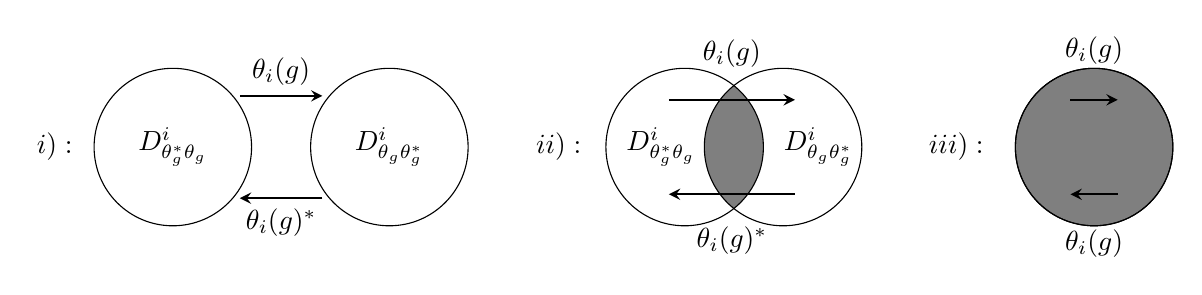
\begin{tikzpicture}
    \begin{scope}[fill opacity=0.5]
         \clip \forthcircle
               \fifthcircle;
     \fill \thirdcircle  
                   \fifthcircle;
    \end{scope}
               
    \draw (-10,0) node {$i):$};  
    \draw \firstcircle node {$D^{i}_{\theta_{g}^{*}\theta_{g}}$};
    \draw \secondcircle node {$D^{i}_{\theta_{g}\theta_{g}^{*}}$};
    \draw[>=stealth,->,thick] (-7.65,0.65) -- node [above] {$\theta_{i}(g)$} (-6.6,0.65);
     \draw[>=stealth,->,thick] (-6.6,-0.65) -- node [below] {$\theta_{i}(g)^{*}$} (-7.65,-0.65);
       
    \draw (-3.6,0) node {$ii):$};  
    \draw \forthcircle ;
    \draw \thirdcircle ;%node  {$D_{g^{*}g$};
    \draw[>=stealth,->,thick] (-2.2,0.6) -- node [above=8pt] {$\theta_{i}(g)$} (-0.6,0.6);
    \draw[>=stealth,->,thick] (-0.6,-0.6) -- node [below=8pt] {$\theta_{i}(g)^{*}$} (-2.2,-0.6);
    \draw (-2.3,0)  node  {$D^{i}_{\theta_{g}^{*}\theta_{g}}$};
    \draw (-0.3,0)  node  {$D^{i}_{\theta_{g}\theta_{g}^{*}}$};
    
    \draw (1.45,0) node {$iii):$};
    \draw \sixthcircle ;
    \draw \fifthcircle;
    \draw[>=stealth,->,thick] (2.9,0.6) --  node [above=9pt] {$\theta_{i}(g)$} (3.5,0.6);
    \draw[>=stealth,->,thick] (3.5,-0.6) --  node [below=9pt] {$\theta_{i}(g)$} (2.9,-0.6);    
    
\end{tikzpicture}
\caption{The three cases for Lemma \ref{Lem:ParFree}}
\end{figure}

Case i) is clear. In Case iii) we observe that $A_{3}:= \sqcup_{i \in I_{3}} D_{\theta_{g}^{*}\theta_{g}}^{i}$ is a stable core. By Lemma \ref{Lem:StabCore}, $\omega\not = \omega_{g}(\omega)$ if $A_{3} \in \omega$. This leaves case ii).

Let $A_{0,i}:= D_{\theta_{g}^{*}\theta_{g}}^{i}\setminus D_{\theta_{g}^{*}\theta_{g}}^{i}\cap D_{\theta_{g}\theta_{g}^{*}}^{i} $ and $A_{1}=D_{\theta_{g}^{*}\theta_{g}}^{i}\cap D_{\theta_{g}\theta_{g}^{*}}^{i}$. Then set $A_{j}=\bigsqcup_{i \in I_{2}}A_{j,i}$ and let $\omega \in \partial \beta X$. If $A_{0} \in \omega$ then $\theta(g)(A_{0})  \subset A_{0}^{c}$, which implies that $\theta(g)(A_{0}) \not \in \theta(g)(\omega)$. 

It remains to deal with $A_{1} \in \omega$. Assume for a contradiction that $\theta(g)(\omega) = \omega$. Then $\theta(g)(A_{1})\cap A_{1} \in \omega$, and we can apply $\theta(g)$ again - denote by $A_{1}^{m}=A_{1} \cap \theta(g)(A_{1}) \cap ... \cap \theta(g)^{m}(A_{1})$. For each $i \in I_{2}$ there exists a power $m_{i}$ of $\theta(g)$ such that this intersection stabilises in $X_{i}$, that is $A_{1,i}^{m_{i}}=A_{1,i}^{m_{i}+1}$. 

Let $\mathcal{A} = \bigcap_{m\in \mathbb{N}} A_{1}^{m}$. This is a stable core. If $\mathcal{A} \in \omega$ then Lemma \ref{Lem:StabCore} gives $\omega \not = \theta_{g}(\omega)$.

So the last case to consider is that $\mathcal{A}^{c}\in \omega$. It suffices to work in $A_{1}$, so let $B_{1}=\mathcal{A}^{c}\cup A_{1}$ and then define $B_{i} = \theta_{g}(B_{i-1})\cap B_{1}$. It follows from the construction of $\mathcal{A}$ that every element $x \in B_{1}$ has an associated smallest natural number $n_{x}$ such that $\theta_{g}^{n_{x}}(x) \not \in B_{n_{x}}$. It is clear from the definition that $B_{i+1} \subset B_{i}$ for every $i$. Lastly, define $B^{-1}_{i+1}:=\theta_{g}^{-1}(B_{i+1}) \subset B_{i}$.  From this we consider the decomposition of $B_{i}$ into two disjoint infinite pieces:
\begin{eqnarray*}
B^{\pm 1}_{i,even}:= \lbrace x \in B_{i}^{\pm 1} | n_{x} \equiv 0 \mbox{ mod } 2 \rbrace \\
B^{\pm 1}_{i,odd}:= \lbrace x \in B_{i}^{\pm 1} | n_{x} \equiv 1 \mbox{ mod } 2 \rbrace.
\end{eqnarray*} 
$\omega$ must choose precisely one of these two pieces for each $i$. Assume without loss that $B_{1,even} \in \omega$. It is clear that $B^{-1}_{2} \cap B_{1,even} = B_{2,even}^{-1} \in \omega$ is sent, by $\theta_{g}$, to $B_{2,odd}$ and so $B_{2,odd} \in \theta_{g}(\omega)$. From the assumption that $\theta_{g}(\omega)=\omega$, we can conclude that $B_{2,odd} \in  \omega$. As ultrafilters are upwardly closed, we know also that $B_{1,odd} \in \omega$, which is a contradiction. 
\end{proof}

This freeness gives us a tool to understand the structure of $S_{\inf}$.

\begin{lemma}\label{Lem:CP}
Let $\lbrace X_{i} \rbrace$ be a sequence of graphs and let $G$ be a group which acts partially on each $X_{i}$. If $G$ fixes any sequence in $\lbrace X_{i} \rbrace$ then the partial action is not free on $\partial \beta X$. 
\end{lemma}
\begin{proof}Let $\theta_{g}$ denote the disjoint union of the $\theta_{g}^{i}$ arising from the partial action of $G$ on each $X_{i}$. To prove this it is enough to show that there is a single $\omega \in\partial\beta X$ that is fixed by the action of some $g \in G$. The hypothesis that $G$ fixes a sequence gives us $\textbf{x}:=\lbrace x_{n} \rbrace_{I}$ with $I$ infinite and $\theta_{g}(\lbrace x_{n} \rbrace) = \lbrace\theta_{g}^{n}(x_{n}) \rbrace_{I} =\lbrace x_{n} \rbrace_{I}$.

Now consider an ultrafilter $\omega \in \partial\beta X$ that picks $\textbf{x}$. Then this ultrafilter $\omega$ is an element of $D_{g^{*}g}$ as $\textbf{x} \subset D_{g^{*}g}$.  Now for any $A \in \omega$ and consider the intersection $A \cap \textbf{x}$. This is fixed by the action of $g$, as it is a subset of $\textbf{x}$. Hence we have: $\theta_{g}(A \cap \textbf{x}) \in \theta_{g}(\omega)$ for every $A \in \omega$. As $\theta_{g}(\omega)$ is an ultrafilter $A \in \theta_{g}(\omega)$, so in particular $\omega \subseteq \theta_{g}(\omega)$, whence $\theta_{g}(\omega)=\omega$. 
\end{proof}

Recall that the inverse monoid $S_{inf}$ is represented geometrically by partial bijections on $I(X)$. This representation gives us access to the geometry of $X$, which we can utilise, in addition to Lemma \ref{Lem:CP}, to understand the structure of $S_{inf}$. 

\begin{lemma}
Consider the inverse monoid $S_{inf}$ as a submonoid of $I(X)$. Then the following hold:
\begin{enumerate}
\item $S_{inf}$ has the property that $g\not = e_{G}$ and $\theta_{g}\not = 0$ implies $theta_{g}$ is not an idempotent; 
\item $S_{inf}$ is $0$-E-unitary;
\item $S_{inf}$ has maximal element set $\lbrace \theta_{g} : g \in F_{k} \rbrace$.
\end{enumerate}
\end{lemma}
\begin{proof}
\hskip
\begin{enumerate}
\item We prove that no non-zero $\theta_{g}$ are idempotent. To do this we pass to the induced action on $\beta X$. We observe that if $\theta_{g}$ is idempotent on $X$ then it extends to an idempotent on $\beta X$, hence on the boundary $\partial \beta X$. $\theta_{g}$ is non-zero implies that there is a non-principal ultrafilter $\omega$ in the domain $\widehat{D}_{\theta_{g}}$. The result then follows from the observation that $\theta_{g}\circ \theta_{g} (\omega) = \theta_{g}(\omega)$ implies that $\theta_{g}$ must now fix the ultrafilter $\theta_{g}(\omega)$, which by Lemma \ref{Lem:ParFree} cannot happen.

\item For 0-E-unitary is is enough to prove that $f \leq \theta_{g}$ implies $\theta_{g} \in E(S)$. Again, we extend the action to $\beta X$. We observe that if $\theta_{g}$ contains an idempotent, then we can build a sequence of elements of $x_{i} \in f \cap \widehat{D}_{\theta_{g}^{*}\theta_{g}} \cap X_{i}$ such that $\theta_{g}$ fixes the sequence, and hence fixes any ultrafilter $\omega$ that picks this sequence by Lemma \ref{Lem:CP}. This is a contradiction, from where we deduce that the only situation for which $f \leq \theta_{g}$ is precisely when $g =e_{G}$ hence trivially $e \leq \theta_{g}$ implies $\theta_{g} \in E(S)$. For the general case, we remark that by the above statement coupled with the dual prehomomorphism property shows that $f \leq s$ implies $s \leq \theta_{e_{G}}$, hence is an idempotent.  

\item We construct the maximal elements. Observe that using the dual prehomomorphism it is clear that every non-zero word $s \in S$ lives below a non-zero $\theta_{g}$. So it is enough to prove that for $\theta_{g}, \theta_{h} \not = 0$, $\theta_{g} \leq \theta_{h} \Rightarrow \theta_{g}=\theta_{h}$. Let $\theta_{g} \leq \theta_{h}$. This translates to $\theta_{h}\theta_{g}^{*}\theta_{g} = \theta_{g}$, hence for all $x \in \widehat{D}_{\theta_{g}^{*}\theta_{g}}: \theta_{h}(x) = \theta_{g}(x)$. Hence $\theta_{g}^{*}\theta_{h} \in E(S)$. From here we see that $\theta_{g}^{*}\theta_{h} \leq \theta_{e}$. From (2) we can deduce: $\theta_{g}^{*}\theta_{h}\leq \theta_{g^{-1}h}$ implies $\theta_{g^{-1}h} \in E(S_{inf})$. By (1) this implies $\theta_{g^{-1}h}=\theta_{e}$, and this happens if and only if $g^{-1}h = e$, i.e $g=h$.\end{proof}
\end{enumerate}

Appealing to the machinery we developed earlier in Propostions \ref{Prop:Strongly} and \ref{Prop:GrpoidHom} we get the following corollary immediately.

\begin{corollary}\label{Cor:MT}
The inverse monoid $S_{inf}$ is strongly 0-F-inverse.
\end{corollary}

We now have enough tools to prove the general version of Theorems \ref{Thm:MR1} and \ref{Thm:MR2}. 

\begin{theorem}
Let $\lbrace X_{i} \rbrace$ be a sequence with large girth and vertex degree uniformly bounded above by $2k$. Let $X$ be the corresponding space of graphs. Then the boundary Baum-Connes conjecture holds for $X$.
\end{theorem}
\begin{proof}
Using Proposition \ref{Prop:Aug} we know the form of the boundary groupoid again in this case: $G(X)|_{\partial\beta X} \cong \partial\beta X \rtimes \G_{\widehat{X}}$. Using results of Tu (namely Theorem 3.13 from \cite{cbcag2}): we know that for any $G(X)|_{\partial\beta X}$-$C^{*}$-algebra $A$ the Baum-Connes conjecture for $G(X)|_{\partial\beta X}$ with coefficients $A$ holds if and only if the conjecture for $\G_{\X}$ with coefficients in $A$ holds. By choosing $A= \frac{\ell^{\infty}(X,\mathcal{K})}{C_{0}(X,\mathcal{K})}$ and remarking that $\G_{\X}$ has the Haagerup property by by Corollary \ref{Cor:MT} and Corollary \ref{Cor:Gpoid} it follows that the boundary coarse Baum-Connes conjecture holds for $X$.
\end{proof}